% Options for packages loaded elsewhere
\PassOptionsToPackage{unicode}{hyperref}
\PassOptionsToPackage{hyphens}{url}
\PassOptionsToPackage{dvipsnames,svgnames,x11names}{xcolor}
%
\documentclass[
]{article}

\usepackage{amsmath,amssymb}
\usepackage{iftex}
\ifPDFTeX
  \usepackage[T1]{fontenc}
  \usepackage[utf8]{inputenc}
  \usepackage{textcomp} % provide euro and other symbols
\else % if luatex or xetex
  \usepackage{unicode-math}
  \defaultfontfeatures{Scale=MatchLowercase}
  \defaultfontfeatures[\rmfamily]{Ligatures=TeX,Scale=1}
\fi
\usepackage{lmodern}
\ifPDFTeX\else  
    % xetex/luatex font selection
\fi
% Use upquote if available, for straight quotes in verbatim environments
\IfFileExists{upquote.sty}{\usepackage{upquote}}{}
\IfFileExists{microtype.sty}{% use microtype if available
  \usepackage[]{microtype}
  \UseMicrotypeSet[protrusion]{basicmath} % disable protrusion for tt fonts
}{}
\usepackage{xcolor}
\usepackage[top=10pc,bottom=10pc,left=11pc,right=11pc,heightrounded]{geometry}
\setlength{\emergencystretch}{3em} % prevent overfull lines
\setcounter{secnumdepth}{-\maxdimen} % remove section numbering

\usepackage{color}
\usepackage{fancyvrb}
\newcommand{\VerbBar}{|}
\newcommand{\VERB}{\Verb[commandchars=\\\{\}]}
\DefineVerbatimEnvironment{Highlighting}{Verbatim}{commandchars=\\\{\}}
% Add ',fontsize=\small' for more characters per line
\usepackage{framed}
\definecolor{shadecolor}{RGB}{241,243,245}
\newenvironment{Shaded}{\begin{snugshade}}{\end{snugshade}}
\newcommand{\AlertTok}[1]{\textcolor[rgb]{0.68,0.00,0.00}{#1}}
\newcommand{\AnnotationTok}[1]{\textcolor[rgb]{0.37,0.37,0.37}{#1}}
\newcommand{\AttributeTok}[1]{\textcolor[rgb]{0.40,0.45,0.13}{#1}}
\newcommand{\BaseNTok}[1]{\textcolor[rgb]{0.68,0.00,0.00}{#1}}
\newcommand{\BuiltInTok}[1]{\textcolor[rgb]{0.00,0.23,0.31}{#1}}
\newcommand{\CharTok}[1]{\textcolor[rgb]{0.13,0.47,0.30}{#1}}
\newcommand{\CommentTok}[1]{\textcolor[rgb]{0.37,0.37,0.37}{#1}}
\newcommand{\CommentVarTok}[1]{\textcolor[rgb]{0.37,0.37,0.37}{\textit{#1}}}
\newcommand{\ConstantTok}[1]{\textcolor[rgb]{0.56,0.35,0.01}{#1}}
\newcommand{\ControlFlowTok}[1]{\textcolor[rgb]{0.00,0.23,0.31}{\textbf{#1}}}
\newcommand{\DataTypeTok}[1]{\textcolor[rgb]{0.68,0.00,0.00}{#1}}
\newcommand{\DecValTok}[1]{\textcolor[rgb]{0.68,0.00,0.00}{#1}}
\newcommand{\DocumentationTok}[1]{\textcolor[rgb]{0.37,0.37,0.37}{\textit{#1}}}
\newcommand{\ErrorTok}[1]{\textcolor[rgb]{0.68,0.00,0.00}{#1}}
\newcommand{\ExtensionTok}[1]{\textcolor[rgb]{0.00,0.23,0.31}{#1}}
\newcommand{\FloatTok}[1]{\textcolor[rgb]{0.68,0.00,0.00}{#1}}
\newcommand{\FunctionTok}[1]{\textcolor[rgb]{0.28,0.35,0.67}{#1}}
\newcommand{\ImportTok}[1]{\textcolor[rgb]{0.00,0.46,0.62}{#1}}
\newcommand{\InformationTok}[1]{\textcolor[rgb]{0.37,0.37,0.37}{#1}}
\newcommand{\KeywordTok}[1]{\textcolor[rgb]{0.00,0.23,0.31}{\textbf{#1}}}
\newcommand{\NormalTok}[1]{\textcolor[rgb]{0.00,0.23,0.31}{#1}}
\newcommand{\OperatorTok}[1]{\textcolor[rgb]{0.37,0.37,0.37}{#1}}
\newcommand{\OtherTok}[1]{\textcolor[rgb]{0.00,0.23,0.31}{#1}}
\newcommand{\PreprocessorTok}[1]{\textcolor[rgb]{0.68,0.00,0.00}{#1}}
\newcommand{\RegionMarkerTok}[1]{\textcolor[rgb]{0.00,0.23,0.31}{#1}}
\newcommand{\SpecialCharTok}[1]{\textcolor[rgb]{0.37,0.37,0.37}{#1}}
\newcommand{\SpecialStringTok}[1]{\textcolor[rgb]{0.13,0.47,0.30}{#1}}
\newcommand{\StringTok}[1]{\textcolor[rgb]{0.13,0.47,0.30}{#1}}
\newcommand{\VariableTok}[1]{\textcolor[rgb]{0.07,0.07,0.07}{#1}}
\newcommand{\VerbatimStringTok}[1]{\textcolor[rgb]{0.13,0.47,0.30}{#1}}
\newcommand{\WarningTok}[1]{\textcolor[rgb]{0.37,0.37,0.37}{\textit{#1}}}

\providecommand{\tightlist}{%
  \setlength{\itemsep}{0pt}\setlength{\parskip}{0pt}}\usepackage{longtable,booktabs,array}
\usepackage{calc} % for calculating minipage widths
% Correct order of tables after \paragraph or \subparagraph
\usepackage{etoolbox}
\makeatletter
\patchcmd\longtable{\par}{\if@noskipsec\mbox{}\fi\par}{}{}
\makeatother
% Allow footnotes in longtable head/foot
\IfFileExists{footnotehyper.sty}{\usepackage{footnotehyper}}{\usepackage{footnote}}
\makesavenoteenv{longtable}
\usepackage{graphicx}
\makeatletter
\def\maxwidth{\ifdim\Gin@nat@width>\linewidth\linewidth\else\Gin@nat@width\fi}
\def\maxheight{\ifdim\Gin@nat@height>\textheight\textheight\else\Gin@nat@height\fi}
\makeatother
% Scale images if necessary, so that they will not overflow the page
% margins by default, and it is still possible to overwrite the defaults
% using explicit options in \includegraphics[width, height, ...]{}
\setkeys{Gin}{width=\maxwidth,height=\maxheight,keepaspectratio}
% Set default figure placement to htbp
\makeatletter
\def\fps@figure{htbp}
\makeatother
% definitions for citeproc citations
\NewDocumentCommand\citeproctext{}{}
\NewDocumentCommand\citeproc{mm}{%
  \begingroup\def\citeproctext{#2}\cite{#1}\endgroup}
\makeatletter
 % allow citations to break across lines
 \let\@cite@ofmt\@firstofone
 % avoid brackets around text for \cite:
 \def\@biblabel#1{}
 \def\@cite#1#2{{#1\if@tempswa , #2\fi}}
\makeatother
\newlength{\cslhangindent}
\setlength{\cslhangindent}{1.5em}
\newlength{\csllabelwidth}
\setlength{\csllabelwidth}{3em}
\newenvironment{CSLReferences}[2] % #1 hanging-indent, #2 entry-spacing
 {\begin{list}{}{%
  \setlength{\itemindent}{0pt}
  \setlength{\leftmargin}{0pt}
  \setlength{\parsep}{0pt}
  % turn on hanging indent if param 1 is 1
  \ifodd #1
   \setlength{\leftmargin}{\cslhangindent}
   \setlength{\itemindent}{-1\cslhangindent}
  \fi
  % set entry spacing
  \setlength{\itemsep}{#2\baselineskip}}}
 {\end{list}}
\usepackage{calc}
\newcommand{\CSLBlock}[1]{\hfill\break\parbox[t]{\linewidth}{\strut\ignorespaces#1\strut}}
\newcommand{\CSLLeftMargin}[1]{\parbox[t]{\csllabelwidth}{\strut#1\strut}}
\newcommand{\CSLRightInline}[1]{\parbox[t]{\linewidth - \csllabelwidth}{\strut#1\strut}}
\newcommand{\CSLIndent}[1]{\hspace{\cslhangindent}#1}

% -----------------------
% CUSTOM PREAMBLE STUFF
% -----------------------

% -----------------
% Typography tweaks
% -----------------
% Indent size
\setlength{\parindent}{1pc}  % 1p0

% Fix widows and orphans
\usepackage[all,defaultlines=2]{nowidow}

% List things
\usepackage{enumitem}
% Same document-level indentation for ordered and ordered lists
\setlist[1]{labelindent=\parindent}
\setlist[itemize]{leftmargin=*}
\setlist[enumerate]{leftmargin=*}

% Wrap definition list terms
% https://tex.stackexchange.com/a/9763/11851
\setlist[description]{style=unboxed}


% For better TOCs
\usepackage[titles]{tocloft}

% Remove left margin in lists inside longtables
% https://tex.stackexchange.com/a/378190/11851
\AtBeginEnvironment{longtable}{\setlist[itemize]{nosep, wide=0pt, leftmargin=*, before=\vspace*{-\baselineskip}, after=\vspace*{-\baselineskip}}}

% Allow for /singlespacing and /doublespacing
\usepackage{setspace}


% -----------------
% Title block stuff
% -----------------

% Abstract
\usepackage[overload]{textcase}
\usepackage[runin]{abstract}
\renewcommand{\abstractnamefont}{\sffamily\footnotesize\bfseries\MakeUppercase}
\renewcommand{\abstracttextfont}{\sffamily\small}
\setlength{\absleftindent}{\parindent * 2}
\setlength{\absrightindent}{\parindent * 2}
\abslabeldelim{\quad}
\setlength{\abstitleskip}{-\parindent}


% Keywords
\newenvironment{keywords}
{\vskip -3em \hspace{\parindent}\small\sffamily{\sffamily\footnotesize\bfseries\MakeUppercase{Keywords}}\quad}
{\vskip 3em}

  
% Title
\usepackage{titling}
\setlength{\droptitle}{3em}
\pretitle{\par\vskip 5em \begin{flushleft}\LARGE\sffamily\bfseries}
\posttitle{\par\end{flushleft}\vskip 0.75em}


% Authors
%
% PHEW this is complicated for a number of reasons!
%
% When using \and with multiple authors, the article class in LaTeX wraps each 
% author block in a tabluar environment with a hardcoded center alignment. It's 
% possible to use \preauthor{} to start tabulars with a left alignment {l}, but 
% that only applies to the first author because the others all use \and with the 
% hardcoded {c}. But we can override the \and command and add our own {l}
%
% (See https://github.com/rstudio/rmarkdown/issues/1716#issuecomment-560601691 
% for an example of redefining \and to just be \\)
%
% That's all great, except tabulars have some amount of default horizontal 
% padding, which makes left-aligned author blocks not actuall get fully 
% left-aligned on the page. We can set the horizontal padding for the column to 
% 0, but it requires some wonky syntax: {@{\hspace{0em}}l@{}}
\renewcommand{\and}{\end{tabular} \hskip 3em \begin{tabular}[t]{@{\hspace{0em}}l@{}}}
\preauthor{\begin{flushleft}
           \lineskip 1.5em 
           \begin{tabular}[t]{@{\hspace{0em}}l@{}}}
\postauthor{\end{tabular}\par\end{flushleft}}

% Omit the date since the \published command does that
\predate{}
\postdate{}

% Command for a note at the top of the first page describing the publication
% status of the paper.
\newcommand{\published}[1]{%
   \gdef\puB{#1}}
   \newcommand{\puB}{}
   \renewcommand{\maketitlehooka}{%
       \par\noindent\footnotesize\sffamily \puB}


% ------------------
% Section headings
% ------------------
\usepackage{titlesec}
\titleformat*{\section}{\Large\sffamily\bfseries\raggedright}
\titleformat*{\subsection}{\large\sffamily\bfseries\raggedright}
\titleformat*{\subsubsection}{\normalsize\sffamily\bfseries\raggedright}
\titleformat*{\paragraph}{\small\sffamily\bfseries\raggedright}

% \titlespacing{<command>}{<left>}{<before-sep>}{<after-sep>}
% Starred version removes indentation in following paragraph
\titlespacing*{\section}{0em}{2em}{0.1em}
\titlespacing*{\subsection}{0em}{1.25em}{0.1em}
\titlespacing*{\subsubsection}{0em}{0.75em}{0em}


% -----------
% Footnotes
% -----------
% NB: footmisc has to come after setspace and biblatex because of conflicts
\usepackage[bottom, flushmargin]{footmisc}
\renewcommand*{\footnotelayout}{\footnotesize}

\addtolength{\skip\footins}{10pt}    % vertical space between rule and main text
\setlength{\footnotesep}{5pt}  % vertical space between footnotes


% ----------
% Captions
% ----------
\usepackage[font={small,sf}, labelfont={small,sf,bf}]{caption}


% --------
% Macros
% --------
% pandoc will not convert text within \begin{} XXX \end{} to Markdown and will
% treat it as regular TeX. Because of this, it's impossible to do stuff like
% this:

% \begin{landscape}
%
% | One | Two   |
% |-----+-------|
% | my  | table |
% | is  | nice  |
%
% \end{landscape}
%
% Since it'll render like: | One | Two | |—–+——-| | my | table | | is | nice |
% 
% BUT, from this http://stackoverflow.com/a/41945462/120898 we can get around
% this by creating new commands for \begin and \end, like this:
\usepackage{pdflscape}
\newcommand{\blandscape}{\begin{landscape}}
\newcommand{\elandscape}{\end{landscape}}

% \blandscape
%
% | One | Two   |
% |-----+-------|
% | my  | table |
% | is  | nice  |
%
% \elandscape

% Same thing, but for generic groups
% But can't use \bgroup and \egroup because those are built-in TeX things
\newcommand{\stgroup}{\begingroup}
\newcommand{\fingroup}{\endgroup}


% ---------------------------
% END CUSTOM PREAMBLE STUFF
% ---------------------------
\makeatletter
\@ifpackageloaded{caption}{}{\usepackage{caption}}
\AtBeginDocument{%
\ifdefined\contentsname
  \renewcommand*\contentsname{Table of contents}
\else
  \newcommand\contentsname{Table of contents}
\fi
\ifdefined\listfigurename
  \renewcommand*\listfigurename{List of Figures}
\else
  \newcommand\listfigurename{List of Figures}
\fi
\ifdefined\listtablename
  \renewcommand*\listtablename{List of Tables}
\else
  \newcommand\listtablename{List of Tables}
\fi
\ifdefined\figurename
  \renewcommand*\figurename{Figure}
\else
  \newcommand\figurename{Figure}
\fi
\ifdefined\tablename
  \renewcommand*\tablename{Table}
\else
  \newcommand\tablename{Table}
\fi
}
\@ifpackageloaded{float}{}{\usepackage{float}}
\floatstyle{ruled}
\@ifundefined{c@chapter}{\newfloat{codelisting}{h}{lop}}{\newfloat{codelisting}{h}{lop}[chapter]}
\floatname{codelisting}{Listing}
\newcommand*\listoflistings{\listof{codelisting}{List of Listings}}
\makeatother
\makeatletter
\makeatother
\makeatletter
\@ifpackageloaded{caption}{}{\usepackage{caption}}
\@ifpackageloaded{subcaption}{}{\usepackage{subcaption}}
\makeatother

\ifLuaTeX
  \usepackage{selnolig}  % disable illegal ligatures
\fi
\usepackage{bookmark}

\IfFileExists{xurl.sty}{\usepackage{xurl}}{} % add URL line breaks if available
\urlstyle{same} % disable monospaced font for URLs
\hypersetup{
  pdftitle={Technocrats to Tycoons},
  pdfauthor={Jonathan Jayes},
  colorlinks=true,
  linkcolor={DarkSlateBlue},
  filecolor={Maroon},
  citecolor={DarkSlateBlue},
  urlcolor={DarkSlateBlue},
  pdfcreator={LaTeX via pandoc}}


% -----------------------
% END-OF-PREAMBLE STUFF
% -----------------------



% ---------------------- 
% Title block elements
% ---------------------- 
\usepackage{orcidlink}  % Create automatic ORCID icons/links

\title{Technocrats to Tycoons}

\usepackage{etoolbox}
\makeatletter
\providecommand{\subtitle}[1]{% add subtitle to \maketitle
  \apptocmd{\@title}{\par {\vskip 0.25em \large #1 \par}}{}{}
}
\makeatother
\subtitle{The Shift in Swedish Corporate Leadership and Its Economic
Consequences in the 20th century}

\author{
{\large Jonathan Jayes~\orcidlink{0000-0003-4967-4869}}%
 \\%
Lund University Economic History Department \\%
{\footnotesize \url{jonathan.jayes@ekh.lu.se}} \and
}

\date{}


% Typeset URLs in the same font as their parent environment
%
% This has to come at the end of the preamble, after any biblatex stuff because 
% some biblatex styles (like APA) define their own \urlstyle{}
\usepackage{url}
\urlstyle{same}

% ---------------------------
% END END-OF-PREAMBLE STUFF
% ---------------------------
\begin{document}
% ---------------
% TITLE SECTION
% ---------------
\published{\textbf{Tuesday, March 4, 2025} \\ {\scriptsize Access the
code, data, and analysis at
\url{https://github.com/j-jayes/who-is-who-etl} and
\url{https://github.com/j-jayes/Swedish-annual-reports-archive}}}

\maketitle



% -------------------
% END TITLE SECTION
% -------------------



Paper structure:

\subsection{I. Introduction}\label{i.-introduction}

\begin{enumerate}
\def\labelenumi{\arabic{enumi}.}
\tightlist
\item
  \textbf{Context and Motivation}

  \begin{itemize}
  \tightlist
  \item
    Briefly outline Sweden's early 20th-century industrial context (high
    reliance on manufacturing and engineering-driven growth).\\
  \item
    Emphasize the role of returning U.S.-experienced engineers as
    carriers of both technical and managerial innovations.\\
  \item
    Highlight the importance of board composition in shaping firm
    performance and industrial employment trajectories.
  \end{itemize}
\item
  \textbf{Research Questions}

  \begin{itemize}
  \tightlist
  \item
    \textbf{Main:} ``How did the presence (and network influence) of
    U.S.-experienced engineers on Swedish boards affect firms' financial
    performance and the evolution of workforce size (especially revenue
    per employee) between the early 20th century and 1980?''\\
  \item
    \textbf{Sub-question:} ``Does the effect differ when comparing
    engineer-trained directors (especially those with U.S. experience)
    to business/finance-trained directors?''
  \end{itemize}
\item
  \textbf{Contribution and Significance}

  \begin{itemize}
  \tightlist
  \item
    Position the study in economic history, corporate governance, and
    labor/employment literatures.\\
  \item
    Stress novelty in using digitized historical data, integrating board
    composition with firm performance metrics \emph{and} bipartite
    network analysis.
  \end{itemize}
\item
  \textbf{Outline of the Paper}

  \begin{itemize}
  \tightlist
  \item
    Summarize each main section:

    \begin{enumerate}
    \def\labelenumii{\arabic{enumii}.}
    \tightlist
    \item
      \textbf{Literature Review} -- situates the question in prior
      scholarship on returning engineers, board composition, and
      technical change/employment.\\
    \item
      \textbf{Data \& Source Criticism} -- details firm-level
      financials, board rosters, and biographical info on directors,
      plus concerns about digitization accuracy.\\
    \item
      \textbf{Empirical Method} -- describes regression approach,
      bipartite network modeling, key variables, and potential
      confounders.\\
    \item
      \textbf{Analysis (not included here yet)} -- presents descriptive
      statistics, network visualizations, and regression results.\\
    \item
      \textbf{Conclusion} -- interprets findings, discusses limitations,
      and proposes avenues for future research.
    \end{enumerate}
  \end{itemize}
\end{enumerate}

\begin{center}\rule{0.5\linewidth}{0.5pt}\end{center}

\subsection{II. Literature Review}\label{ii.-literature-review}

\begin{enumerate}
\def\labelenumi{\arabic{enumi}.}
\tightlist
\item
  \textbf{Returning Engineers, Technology Transfer, and Organizational
  Change}

  \begin{itemize}
  \tightlist
  \item
    Grönberg (2003) on the ``brain gain'' phenomenon: how U.S. exposure
    spurred Swedish industrial development via both technology and
    managerial innovations.\\
  \item
    Broader literature on knowledge spillovers and rationalization
    (Taylorism, mass-production methods, etc.) introduced by
    internationally trained engineers.
  \end{itemize}
\item
  \textbf{Boards, Governance, and Firm Performance}

  \begin{itemize}
  \tightlist
  \item
    Overview of corporate governance research linking board composition
    to firm outcomes (late 20th- and 21st-century focus, typically).\\
  \item
    Gaps in historical analysis (turn of the 20th century to
    \textasciitilde1980) due to data availability.\\
  \item
    Emergence of interest in network ties (director interlocks,
    ``Wallenberg sphere,'' etc.) and how these can diffuse managerial
    practices.
  \end{itemize}
\item
  \textbf{Technical Change, Employment, and Revenue per Employee}

  \begin{itemize}
  \tightlist
  \item
    Literature on the relationship between technology adoption and labor
    dynamics, e.g.~how new technology can boost productivity or displace
    labor.\\
  \item
    Historical perspectives on Sweden's strong manufacturing base and
    how productivity growth contributed to relatively high growth and
    lower inequality (Molinder \& Prado).\\
  \item
    Relevance to the study of ``revenue per employee'' as a measure of
    labor productivity over time.
  \end{itemize}
\item
  \textbf{Engineers vs.~Business/Finance Directors} (Sub-Question Focus)

  \begin{itemize}
  \tightlist
  \item
    Discussion of the distinct skill sets: engineers bringing
    technical/operational expertise vs.~business/finance directors
    focusing on strategic, financial control.\\
  \item
    Potential complementary roles, but also potential differences in how
    each group influences investment in new technologies or workforce
    expansion/contraction.\\
  \item
    Preliminary insights from research indicating that foreign-trained
    engineers may enjoy faster career advancement and implement more
    radical innovations.
  \end{itemize}
\item
  \textbf{Research Gap and Positioning}

  \begin{itemize}
  \tightlist
  \item
    Despite parallel lines of research, few studies combine historical
    board-level data with long-run performance/employment outcomes and
    network analysis.\\
  \item
    Your project addresses this gap by drawing on newly digitized
    company records, board rosters, and individual biographies.
  \end{itemize}
\end{enumerate}

\begin{center}\rule{0.5\linewidth}{0.5pt}\end{center}

\subsection{III. Data and Source
Criticism}\label{iii.-data-and-source-criticism}

\begin{enumerate}
\def\labelenumi{\arabic{enumi}.}
\tightlist
\item
  \textbf{Data Sources}

  \begin{itemize}
  \tightlist
  \item
    \textbf{Firm-Level Financials} (1900--1980): Revenue, profits,
    number of employees, possibly other controls (industry
    classification, capital structure).\\
  \item
    \textbf{Board Composition}: 71 firms for which you have rosters of
    board members, including name, tenure, and professional
    background.\\
  \item
    \textbf{Biographical Details of Directors}: Education (technical
    vs.~business), foreign experience (U.S. or elsewhere), social
    background, etc.
  \end{itemize}
\item
  \textbf{Data Collection and Digitization}

  \begin{itemize}
  \tightlist
  \item
    Outline the process of digitizing archival company reports; note any
    challenges in scanning, OCR errors, or partial coverage.\\
  \item
    Summarize how you consolidated multiple archival sources into a
    single dataset (e.g., matching board-member rosters across time,
    linking to finance data).
  \end{itemize}
\item
  \textbf{Source Criticism}

  \begin{itemize}
  \tightlist
  \item
    \textbf{Completeness and Representativeness}: Are the 71 firms a
    representative cross-section of Swedish industry? Are they skewed
    toward large manufacturing concerns or spread across different
    sectors (including banks)?\\
  \item
    \textbf{Accuracy of Biographical Info}: Potential biases in
    self-reported career histories or incomplete records on foreign
    experience.\\
  \item
    \textbf{Temporal Inconsistencies}: Different firms may report
    financial data on different cycles or with distinct accounting
    standards, especially over 80 years.
  \end{itemize}
\item
  \textbf{Operationalizing Key Variables}

  \begin{itemize}
  \tightlist
  \item
    \textbf{Presence of U.S.-Trained Engineer on the Board}: Binary?
    Count or proportion of total board seats? Weighted by the number of
    years spent abroad?\\
  \item
    \textbf{Engineer vs.~Business/Finance Directors}: Distilling
    multiple educational/training backgrounds into consistent
    categories.\\
  \item
    \textbf{Firm Performance Measures}: Revenue per employee, also
    consider profit margin or ROI for robustness.\\
  \item
    \textbf{Network Measures}: Board interlocks, centrality in the
    bipartite network, etc.
  \end{itemize}
\item
  \textbf{Ethical and Privacy Considerations}

  \begin{itemize}
  \tightlist
  \item
    Historical dataset typically exempt from modern privacy concerns,
    but note any possible issues in naming individuals or citing
    personal details.
  \end{itemize}
\end{enumerate}

\begin{center}\rule{0.5\linewidth}{0.5pt}\end{center}

\subsection{IV. Empirical Method}\label{iv.-empirical-method}

\begin{enumerate}
\def\labelenumi{\arabic{enumi}.}
\tightlist
\item
  \textbf{Overall Study Design}

  \begin{itemize}
  \tightlist
  \item
    \textbf{Longitudinal/Panel Approach}: Observing changes in board
    composition and firm outcomes over time, controlling for firm fixed
    effects.\\
  \item
    \textbf{Bipartite Network Model}: Describing the construction of the
    firm--board-member network, how to transform it into relevant
    metrics (e.g., shared directors).
  \end{itemize}
\item
  \textbf{Regression Specifications}

  \begin{itemize}
  \tightlist
  \item
    Outline separate (or combined) regression equations:

    \begin{enumerate}
    \def\labelenumii{\arabic{enumii}.}
    \tightlist
    \item
      \textbf{Firm Performance Equation}: Dependent variable = (
      \text{Revenue per employee}\_\{i,t\} ) (or alternative).
      Independent variables include:

      \begin{itemize}
      \tightlist
      \item
        Presence/proportion of U.S.-experienced engineers on the board\\
      \item
        Interaction between engineers and foreign experience\\
      \item
        Basic controls (firm age, size, industry fixed effects, economic
        cycle dummies)\\
      \end{itemize}
    \item
      \textbf{Employment Equation} (optional or combined with
      performance): Dependent variable might be total employees or
      growth in employees, same key regressors.\\
    \end{enumerate}
  \item
    For the sub-question: interactions between engineer-trained
    vs.~business/finance directors, with/without U.S. experience.
  \end{itemize}
\item
  \textbf{Network Analysis}

  \begin{itemize}
  \tightlist
  \item
    \textbf{Bipartite Representation}: Firms on one side; directors on
    the other.\\
  \item
    \textbf{Key Metrics}:

    \begin{itemize}
    \tightlist
    \item
      Degree centrality of a director (how many boards they sit on).\\
    \item
      Firm connectivity (how many directors in common with other
      firms).\\
    \item
      Clustering of ``engineer-heavy'' boards in certain industrial
      clusters (e.g., the ``Wallenberg sphere'').\\
    \end{itemize}
  \item
    \textbf{Hypothesized Effects}: More central or more
    ``engineer-heavy'' boards could diffuse similar practices or
    reinforce productivity gains.
  \end{itemize}
\item
  \textbf{Addressing Potential Endogeneity}

  \begin{itemize}
  \tightlist
  \item
    Discussion of possible reverse causality (e.g., high-performing
    firms attract high-profile directors).\\
  \item
    If available, mention instrumental variables or ``timing''
    arguments---new board appointments are determined partly by
    generational turnover, which might be exogenous to short-run
    performance.\\
  \item
    Alternatively, use lagged values of board composition or
    difference-in-differences if a plausible ``shock'' is identifiable.
  \end{itemize}
\item
  \textbf{Robustness Checks}

  \begin{itemize}
  \tightlist
  \item
    Consider alternative specifications (e.g., panel fixed effects,
    random effects).\\
  \item
    Examine whether results hold for different sub-periods (pre-1930
    vs.~post-1945) or different industries.
  \end{itemize}
\end{enumerate}

\begin{center}\rule{0.5\linewidth}{0.5pt}\end{center}

\textbf{Next Steps}:

\begin{itemize}
\tightlist
\item
  \textbf{Section V. Analysis} (to follow)

  \begin{itemize}
  \tightlist
  \item
    Descriptive stats: distribution of board-member backgrounds,
    proportion of returning engineers over time, correlations among key
    variables.\\
  \item
    Visualizations of the bipartite network (or its unipartite
    projections).\\
  \item
    Regression results and interpretation of coefficients, especially
    focusing on the difference between engineer-trained
    vs.~business-trained directors.\\
  \item
    Potential historical case studies to illustrate ``mechanisms''
    behind the empirical patterns.
  \end{itemize}
\end{itemize}

\subsection{II. Literature Review}\label{ii.-literature-review-1}

\subsubsection{Engineers and Technological Change in Swedish
Industry}\label{engineers-and-technological-change-in-swedish-industry}

Engineers played a pivotal role in Sweden's rapid industrialization and
the management of its early 20th-century firms. As Sweden's industries
expanded in technical complexity (steel, electrification, machinery),
professional engineers increasingly assumed top managerial
roles\hspace{0pt}
(\citeproc{ref-hogfeldt2005HistoryPoliticsCorporate}{Högfeldt 2005}).
Many large firms by the 1920s were effectively run by engineer-CEOs with
significant autonomy, reflecting the technocratic character of Swedish
industry. Business historians note that engineers dominated executive
positions in Sweden's biggest firms, especially in industrial sectors --
highlighting the historical importance of technical training in
corporate leadership
(\citeproc{ref-henrekson2021SocialBackgroundElite}{Henrekson,
Lyssarides, and Ottosson 2021}). This contrasts with some other
countries where legal or financial elites held sway; in Sweden the
engineering profession emerged as a powerful elite driving industrial
growth\hspace{0pt}, according to Henrekson, Lyssarides, and Ottosson
(\citeproc{ref-henrekson2021SocialBackgroundElite}{2021}).

A distinctive feature of Swedish industrialization was the influence of
engineers who trained or worked abroad, particularly in the United
States. Studies of return migration find that a ``brain gain'' occurred:
a majority of Swedish engineers who went to the U.S. (or Germany) for
experience later returned home, bringing valuable knowledge\hspace{0pt}
(\citeproc{ref-gronberg2003LearningReturningReturn}{Grönberg 2003}).
Per-Olof Grönberg's seminal work (2003) shows these returnee engineers
diffused advanced technologies and organizational innovations into
Swedish firms during the country's ``second industrial
breakthrough''\hspace{0pt}, as coined by Lars Magnusson
(\citeproc{ref-magnusson2014SverigesEkonomiskaHistoria}{2014}). They not
only introduced new technical expertise but also modern management
practices -- notably Taylorist efficient workflows and corporate welfare
programs learned in America\hspace{0pt}, according to Grönberg
(\citeproc{ref-gronberg2003LearningReturningReturn}{2003}). For example,
at electrical firm ASEA and steelmaker Sandvik, foreign-trained
engineers filled many key positions, injecting know-how that
rationalized production and improved productivity\hspace{0pt}.
\hspace{0pt} By the early 1900s Swedish industry actively encouraged
this knowledge transfer: contemporary observers remarked that American
and German experience became a form of ``symbolic capital'' that boosted
engineers' influence in firms\hspace{0pt}
(\citeproc{ref-gronberg2003LearningReturningReturn}{Grönberg 2003}).
Case studies confirm that returning engineers were catalysts for
technology diffusion -- from mining equipment to electrotechnical
systems -- adapting foreign innovations to domestic needs\hspace{0pt}.
In sum, engineer-entrepreneurs and internationally trained technologists
were central to Sweden's technological adoption and industrial
leadership in the first three-quarters of the 20th century.

Historians have documented specific instances of how engineers spurred
technological change. For example, Hugo Hammar (an engineer-CEO of
shipbuilder Götaverken) leveraged political and donor networks to fund
naval technology experiments, illustrating how engineering know-how
combined with savvy management advanced key industries\hspace{0pt}
(\citeproc{ref-gronberg2003LearningReturningReturn}{Grönberg 2003}).
Swedish engineers abroad often studied cutting-edge methods and upon
return implemented them -- such as advanced steel processes or
automotive designs -- in their firms\hspace{0pt}. This ``reverse
technology transfer'' was a key mechanism for Sweden's industrial
upgrading, as engineers brought back not just blueprints but also new
organizational structures and quality control systems\hspace{0pt}.
Grönberg notes that engineers coming back from U.S. firms frequently
brought home a welfare capitalist ethos (company housing, worker
benefits) along with efficiency methods. The impact of these returning
engineers on firm performance and workforce dynamics, however, remains
underexplored.

\subsubsection{Board Composition and Corporate
Governance}\label{board-composition-and-corporate-governance}

Historically, Sweden's corporate governance has been characterized by
concentrated ownership and technocratic management, which influenced
board composition and firm performance. In the early 20th century, many
industrial companies were founded by inventors or families but
eventually came under bank or holding-company control\hspace{0pt}. Banks
like Stockholms Enskilda (Wallenberg family) became dominant
shareholders and placed representatives on boards, maintaining close
control of the firm
(\citeproc{ref-hogfeldt2005HistoryPoliticsCorporate}{Högfeldt 2005}).
This led to boards that mixed financiers (owners or bankers) with career
engineers in top executive roles. As Högfeldt
(\citeproc{ref-hogfeldt2005HistoryPoliticsCorporate}{2005}) notes, given
the technically advanced nature of Swedish manufacturing firms,
banks-owners TODO ``lacked the competence to run the firms themselves,''
so they installed engineer-managers and oversaw as active
owners\hspace{0pt}. By the 1950s, an interesting governance model had
emerged: the CEO (often an engineer) held a very strong position,
sometimes even outmaneuvering controlling shareholders by rallying
minority investors\hspace{0pt}. In effect, Swedish boards functioned
with a balance between the technical expertise of managers and the
financial oversight of owners, a structure somewhat distinct from the
purely managerial or family-dominated models elsewhere.

Research on board composition generally finds it can significantly
affect firm outcomes, and this has both historical and modern
dimensions. For instance, a recent study of Swedish companies in the
21st century noted that larger board size correlates with weaker
financial performance (possibly due to coordination
difficulties)\hspace{0pt}
(\citeproc{ref-jonsson2015CorporateBoardsPerformance}{Jönsson 2015}).
This suggests that even historically, leaner governance structures might
have benefited firms in Sweden's relatively concentrated ownership
environment. Board expertise and background also matter: in Sweden, many
directors and CEOs throughout the mid-20th century had engineering or
science educations, whereas later decades saw more with business or
finance degrees, as noted by Henrekson, Lyssarides, and Ottosson
(\citeproc{ref-henrekson2021SocialBackgroundElite}{2021}), who study the
chief executives of the 30 largest firms in Sweden in the 20th century.
They find in their analysis of top Swedish CEOs over 1945--2005, a large
share held engineering degrees, although by the late 20th century it
became common to couple technical training with business
education\hspace{0pt}. This mix of backgrounds on boards can influence
corporate strategy -- technically trained directors may prioritize R\&D
and long-term product development, while finance-trained directors might
emphasize cost control, acquisitions, or shareholder returns.
Comparative studies support this notion: for example, Adams, Hermalin,
and Weisbach (\citeproc{ref-adams2010RoleBoardsDirectors}{2010}) finds
TODO. (\citeproc{ref-asahak2018BoardsDirectorsAssessing}{Asahak et al.
2018}) TODO.

In terms of governance models, Högfeldt
(\citeproc{ref-hogfeldt2005HistoryPoliticsCorporate}{2005}) argues that
Sweden has been seen as a coordinated market economy with
stakeholder-oriented governance, in contrast to the Anglo-American
shareholder model. Throughout the 20th century, Swedish boards were
typically insider-dominated, featuring controlling shareholders or their
proxies (e.g.~the Wallenberg family members) alongside key executives.
This is akin to continental European practices (e.g.~German universal
banks and interlocking directorates)\hspace{0pt}. By the late 1900s,
however, some convergence occurred. Sluyterman and Westerhuis
(\citeproc{ref-sluyterman2022ChangingRoleCEOs}{2022}), studying the
changing role of CEOs in the second half of the 20th century note a
general shift in many countries from ``managerial capitalism'' -- where
industrial experts and managers had primacy -- to ``investor
capitalism'' focused on shareholders\hspace{0pt}. In Sweden, the 1980s
and 1990s brought reforms (e.g.~a Corporate Governance Code) emphasizing
board independence and accountability, more similar to U.S./UK
practices\hspace{0pt}, according to Sabelfeld and Jonäll
(\citeproc{ref-sabelfeld2023SwedishCorporateGovernance}{2023}). Still,
differences remain: Swedish boards to this day often include employee
representatives and maintain high ownership concentration via dual-class
shares and family foundations\hspace{0pt}
(\citeproc{ref-hogfeldt2005HistoryPoliticsCorporate}{Högfeldt 2005}).

Historically, an engineering-trained director in Sweden wielded
influence through deep firm-specific knowledge, whereas a
finance-trained director might exert influence through external networks
and capital access. The interplay of these skills on boards has been
crucial. For instance, Marcus Wallenberg Sr.~in 1905 highlighted that
Sweden had ``able engineers and good workers but lacked entrepreneurs,''
proposing to educate more businesspeople and let banks invest in
industry\hspace{0pt}
(\citeproc{ref-hogfeldt2005HistoryPoliticsCorporate}{Högfeldt 2005}).
This led to a governance system that deliberately blended technical and
financial leadership. Overall, the literature suggests that a balanced
board -- combining technical expertise with financial oversight -- was
key to robust firm performance in Sweden's high-growth era, and
governance structures evolved to institutionalize that balance.

\subsubsection{Firm Performance and Technical
Change}\label{firm-performance-and-technical-change}

The composition of a firm's leadership and board can significantly
influence its performance, especially during periods of technological
change. A growing body of evidence links board composition (skills,
size, and diversity of directors) to financial outcomes like
productivity and profitability. For example, firms that appoint
directors with relevant industry or technical expertise tend to see
positive market reactions and long-run results. von Meyerinck, Oesch,
and Schmid
(\citeproc{ref-vonmeyerinck2016DirectorIndustryExperience}{2016}), who
conducted a study of S\&P 500 companies found that adding a new director
with industry experience led to significantly higher stock price gains
around the announcement. This suggests that specialized knowledge --
such as engineering know-how in a tech-driven company -- is valued by
investors and likely helps firm performance. Likewise, upper-echelon
research indicates that executives' educational backgrounds can shape
firm strategy. CEOs with science/engineering training are often more
innovation-oriented, correlating with greater R\&D investment and
patenting activity
(\citeproc{ref-ghardallou2020CEOCharacteristicsFirm}{Ghardallou, Borgi,
and Alkhalifah 2020}). In fact, Hambrick \& Mason's theory of managerial
characteristics influencing outcomes is supported by findings that
``firm R\&D spending is positively related to the science and
engineering education of its CEO''\hspace{0pt}
(\citeproc{ref-ghardallou2020CEOCharacteristicsFirm}{Ghardallou, Borgi,
and Alkhalifah 2020}). This implies that when technical experts lead
firms, they tend to allocate more resources to innovation, potentially
driving productivity growth. Conversely, leaders with primarily
financial backgrounds might focus on efficiency metrics and short-term
returns, affecting measures like revenue per employee or labor costs in
different ways.

Historical analyses of Swedish companies provide empirical insight into
how technical leadership affected performance and employment. During
Sweden's era of industrial ascendancy (roughly 1900--1970), many firms
achieved world-class productivity levels. By 1950, Sweden had caught up
with some of the richest nations in GDP per capita -- a feat usually
credited to its manufacturing industries' success in adopting and
advancing frontier technology\hspace{0pt}, as summarized by Prado and
Molinder (\citeproc{ref-prado2022ModernSwedishEconomic}{2022}). Within
manufacturing, engineer-led firms introduced process improvements and
new products that boosted output per worker. Indeed, from 1950 to 1970
Swedish manufacturing output grew about 4.8\% annually, contributing
more than half of national GDP growth in that ``golden age'', as noted
by Taalbi and Ljungberg
(\citeproc{ref-taalbiInnovationsEconomicGrowth}{n.d.})\hspace{0pt}.
Firms like ASEA (electrical equipment) or Volvo (automotive) saw rapid
productivity gains as they implemented technical innovations and modern
management, often under the guidance of technically trained executives.
Revenue per employee and related metrics rose as these companies scaled
up and optimized production. However, the link between technical change
and employment is complex. In the early and mid-20th century, industrial
employment expanded alongside productivity -- manufacturing employment
kept rising up to the 1960s as firms grew\hspace{0pt}
(\citeproc{ref-taalbiInnovationsEconomicGrowth}{Taalbi and Ljungberg,
n.d.}). High productivity and output often went hand in hand with more
jobs during this expansion phase.

After the 1970s, a shift occurred in performance dynamics, illustrating
the impact of technological transformation on employment. As Sweden and
other advanced economies faced the ICT revolution and globalization,
manufacturing employment peaked and then ``deindustrialization'' set
in\hspace{0pt}. Automation and technical efficiencies meant output could
keep growing with fewer workers. For Sweden, the period 1970--1990 saw
manufacturing value-added growth drop to about 1.5\% per year (from
\textasciitilde4.8\% earlier), and the sector's share of total growth
fell markedly (\citeproc{ref-taalbiInnovationsEconomicGrowth}{Taalbi and
Ljungberg, n.d.}). Yet manufacturing's productivity continued to improve
-- output did not collapse, it simply required far less labor input. As
Ljungberg and Taalbi note, after 1970 the output of manufacturing kept
rising despite workforce cuts, implying that capital deepening and
technical change drove up labor productivity\hspace{0pt}. The
consequence was a decline in the labor share and industrial employment,
even as firms became more efficient. Corporate governance may have
played a role in this transition: starting in the 1980s, more
financially driven management (sometimes replacing engineer-leaders)
pursued restructuring, outsourcing, and cost reduction to please
shareholders, which often entailed layoffs or wage restraint. Here,
historical data illustrate that technical leadership and board expertise
can yield higher innovation and productivity (raising performance
indicators like revenue per employee or profit margins), but the
distribution of those gains between capital and labor can shift. Early
on, technology-driven growth supported broad employment, whereas later,
rapid technical change improved output while trimming workforces.
Understanding this evolution is crucial, and it highlights why examining
the backgrounds of board members (engineers vs.~businessmen) is key to
interpreting firm strategies on growth, innovation, and employment.

\subsubsection{Network Analysis and Firm
Governance}\label{network-analysis-and-firm-governance}

In recent years, historians and economists have applied bipartite
network analysis to study corporate governance in a historical context.
A bipartite network (two-mode network) is a representation that links
two types of nodes -- for example, companies and their board members --
without direct connections among nodes of the same type
(\citeproc{ref-liew2023MethodologyFrameworkBipartite}{\textbf{liew2023MethodologyFrameworkBipartite?}}).
(\citeproc{ref-pavlopoulos2018BipartiteGraphsSystems}{\textbf{pavlopoulos2018BipartiteGraphsSystems?}})
notes that by projecting such a network, one can derive the inter-firm
director network (directors are connected if they sit on a common board)
or the interlocking firm network (firms are connected if they share a
director). This approach has opened new avenues to quantify how board
interlocks and elite networks influence firm decision-making and
performance\hspace{0pt}. By digitizing century-long board membership
records of Swedish companies\hspace{0pt}, one can identify which
individuals sat on multiple boards and measure their network centrality
(influence). Such quantitative network measures (degree, centrality,
etc.) can then be used as variables in regression models to assess
impact on firm outcomes
(\citeproc{ref-hsieh2022CollaborationBipartiteNetworks}{\textbf{hsieh2022CollaborationBipartiteNetworks?}}).
This method allows us to test, for instance, whether firms that are more
centrally connected in the director network had better financial
performance.

Studies of corporate networks in Sweden reveal a tightly interlocked
business community, historically dominated by a few key ``nodes.''
Perhaps the most famous example is the Wallenberg sphere -- a cluster of
firms linked by the Wallenberg family through ownership and board
positions. By mid-20th century, the Wallenbergs' investment company
Investor AB and affiliated bank (SEB) held significant stakes in
numerous industrial giants (ASEA, Ericsson, SKF, etc.), and Wallenberg
representatives occupied board seats across these companies
(\citeproc{ref-hogfeldt2005HistoryPoliticsCorporate}{Högfeldt 2005}).
This created a dense network of interlocking directorates where a
handful of individuals oversaw multiple firms.
(\citeproc{ref-ottosson1997InterlockingDirectoratesSwedish}{\textbf{ottosson1997InterlockingDirectoratesSwedish?}})
conducts a network analysis that confirms Swedish big business was
highly connected: an analysis of early 1900s interlocks showed that the
rise of modern banking went hand in hand with interlinked boards in
industry.
(\citeproc{ref-ottosson1997InterlockingDirectoratesSwedish}{\textbf{ottosson1997InterlockingDirectoratesSwedish?}})
's analysis covers five benchmark years; 1903, 1912, 1918, 1924 and
1939, and finds that that Swedish banks became more central actors in
corporate networks over time, especially after financial crises, as they
stepped in to restructure and stabilize industry. By the 1960s, the
three largest banks (Wallenberg's SEB, Handelsbanken, and others) each
had direct or indirect board links to myriad companies, effectively
coordinating corporate strategy in what one commentator called a
``consultation economy''\hspace{0pt}, according to Högfeldt
(\citeproc{ref-hogfeldt2005HistoryPoliticsCorporate}{2005}). Further,
Högfeldt (\citeproc{ref-hogfeldt2005HistoryPoliticsCorporate}{2005})
argues that these inter-firm networks sometimes facilitated resource
sharing, risk management, and technology transfer among companies. For
example, a director sitting on boards of both a steel company and an
engineering firm could help channel investments or collaborative R\&D
between them. Such positive effects of interlocks -- spreading best
practices or providing stable long-term capital -- have been noted in
historical accounts of Swedish conglomerates\hspace{0pt}.

On the other hand, network concentration also meant a small elite could
exert outsized influence.
(\citeproc{ref-dejong2021ExceptionalBigLinkers}{\textbf{dejong2021ExceptionalBigLinkers?}})
mapped Dutch interlocking directorates and found a high degree of
centrality among a few ``big linkers'' (individuals with many board
seats) who could shape multiple firms' decisions. Using modern network
analysis tools on historical data, researchers can evaluate how these
interlocks correlated with firm outcomes. The evidence provided by
(\citeproc{ref-ottosson1997InterlockingDirectoratesSwedish}{\textbf{ottosson1997InterlockingDirectoratesSwedish?}})
in the first half of the 20th century suggests that firms at the core of
interlock networks often had more consistent performance (thanks to
coordinated support during downturns), but overly dense networks might
also stifle competition or innovation if the same directors resisted
change later in the period.

By using a bipartite network analysis based on digitized annual reports
and shareholder registers, I can create a longitudinal panel and yearly
network of board interconnections and then test hypotheses about
governance and performance\hspace{0pt}. Through regression-based network
analysis, it becomes possible to isolate effects: e.g.~did firms with
more connected engineers on their boards achieve higher revenue growth
compared to others? Did a change in board network centrality precede
changes in employment or labor share? That is what I aim to explore in
this paper.

\subsection{III. Data and Source
Criticism}\label{iii.-data-and-source-criticism-1}

\subsubsection{Data sources}\label{data-sources}

This study draws on two interrelated data sources to examine the link
between U.S.-experienced engineers on Swedish corporate boards and
firm-level outcomes; firm-level financials, board composition, and
biographical details of directors. The first two come from company
reports, while the third is extracted from two sets of biographical
dictionaries that detail the lives of prominent Swedes in the 20th
century.

I access the annual reports for companies listed on the Stockholm Stock
Exchange, collected from the online archives of the Swedish House of
Finance at the Stockholm School of Economics (SSE). These reports span
1873--2006, and are provided in PDF form. For the present project, the
focus is on data from 1873 to 1980. I extract from these reports income
statement information including revenue, cost of goods sold, operating
expenses, wages, taxes, depreciation, net income, as well as balance
sheet line items; total assets, current assets, fixed assets, total
liabilities, current liabilities, long-term liabilities, and shareholder
equity. I also extract the number of workers (sometimes disaggregated
into white-collar vs.~blue-collar).

I limit the sample to firms with at least 30 years of data betwen 1873
and 1980, resulting in 71 firms included. For these 71 firms, the annual
reports list the names and positions of their board members (alongside
auditors) near the balance sheet. Figure~\ref{fig-crot} displays the
coverage by firm and year.

\begin{figure}

\centering{

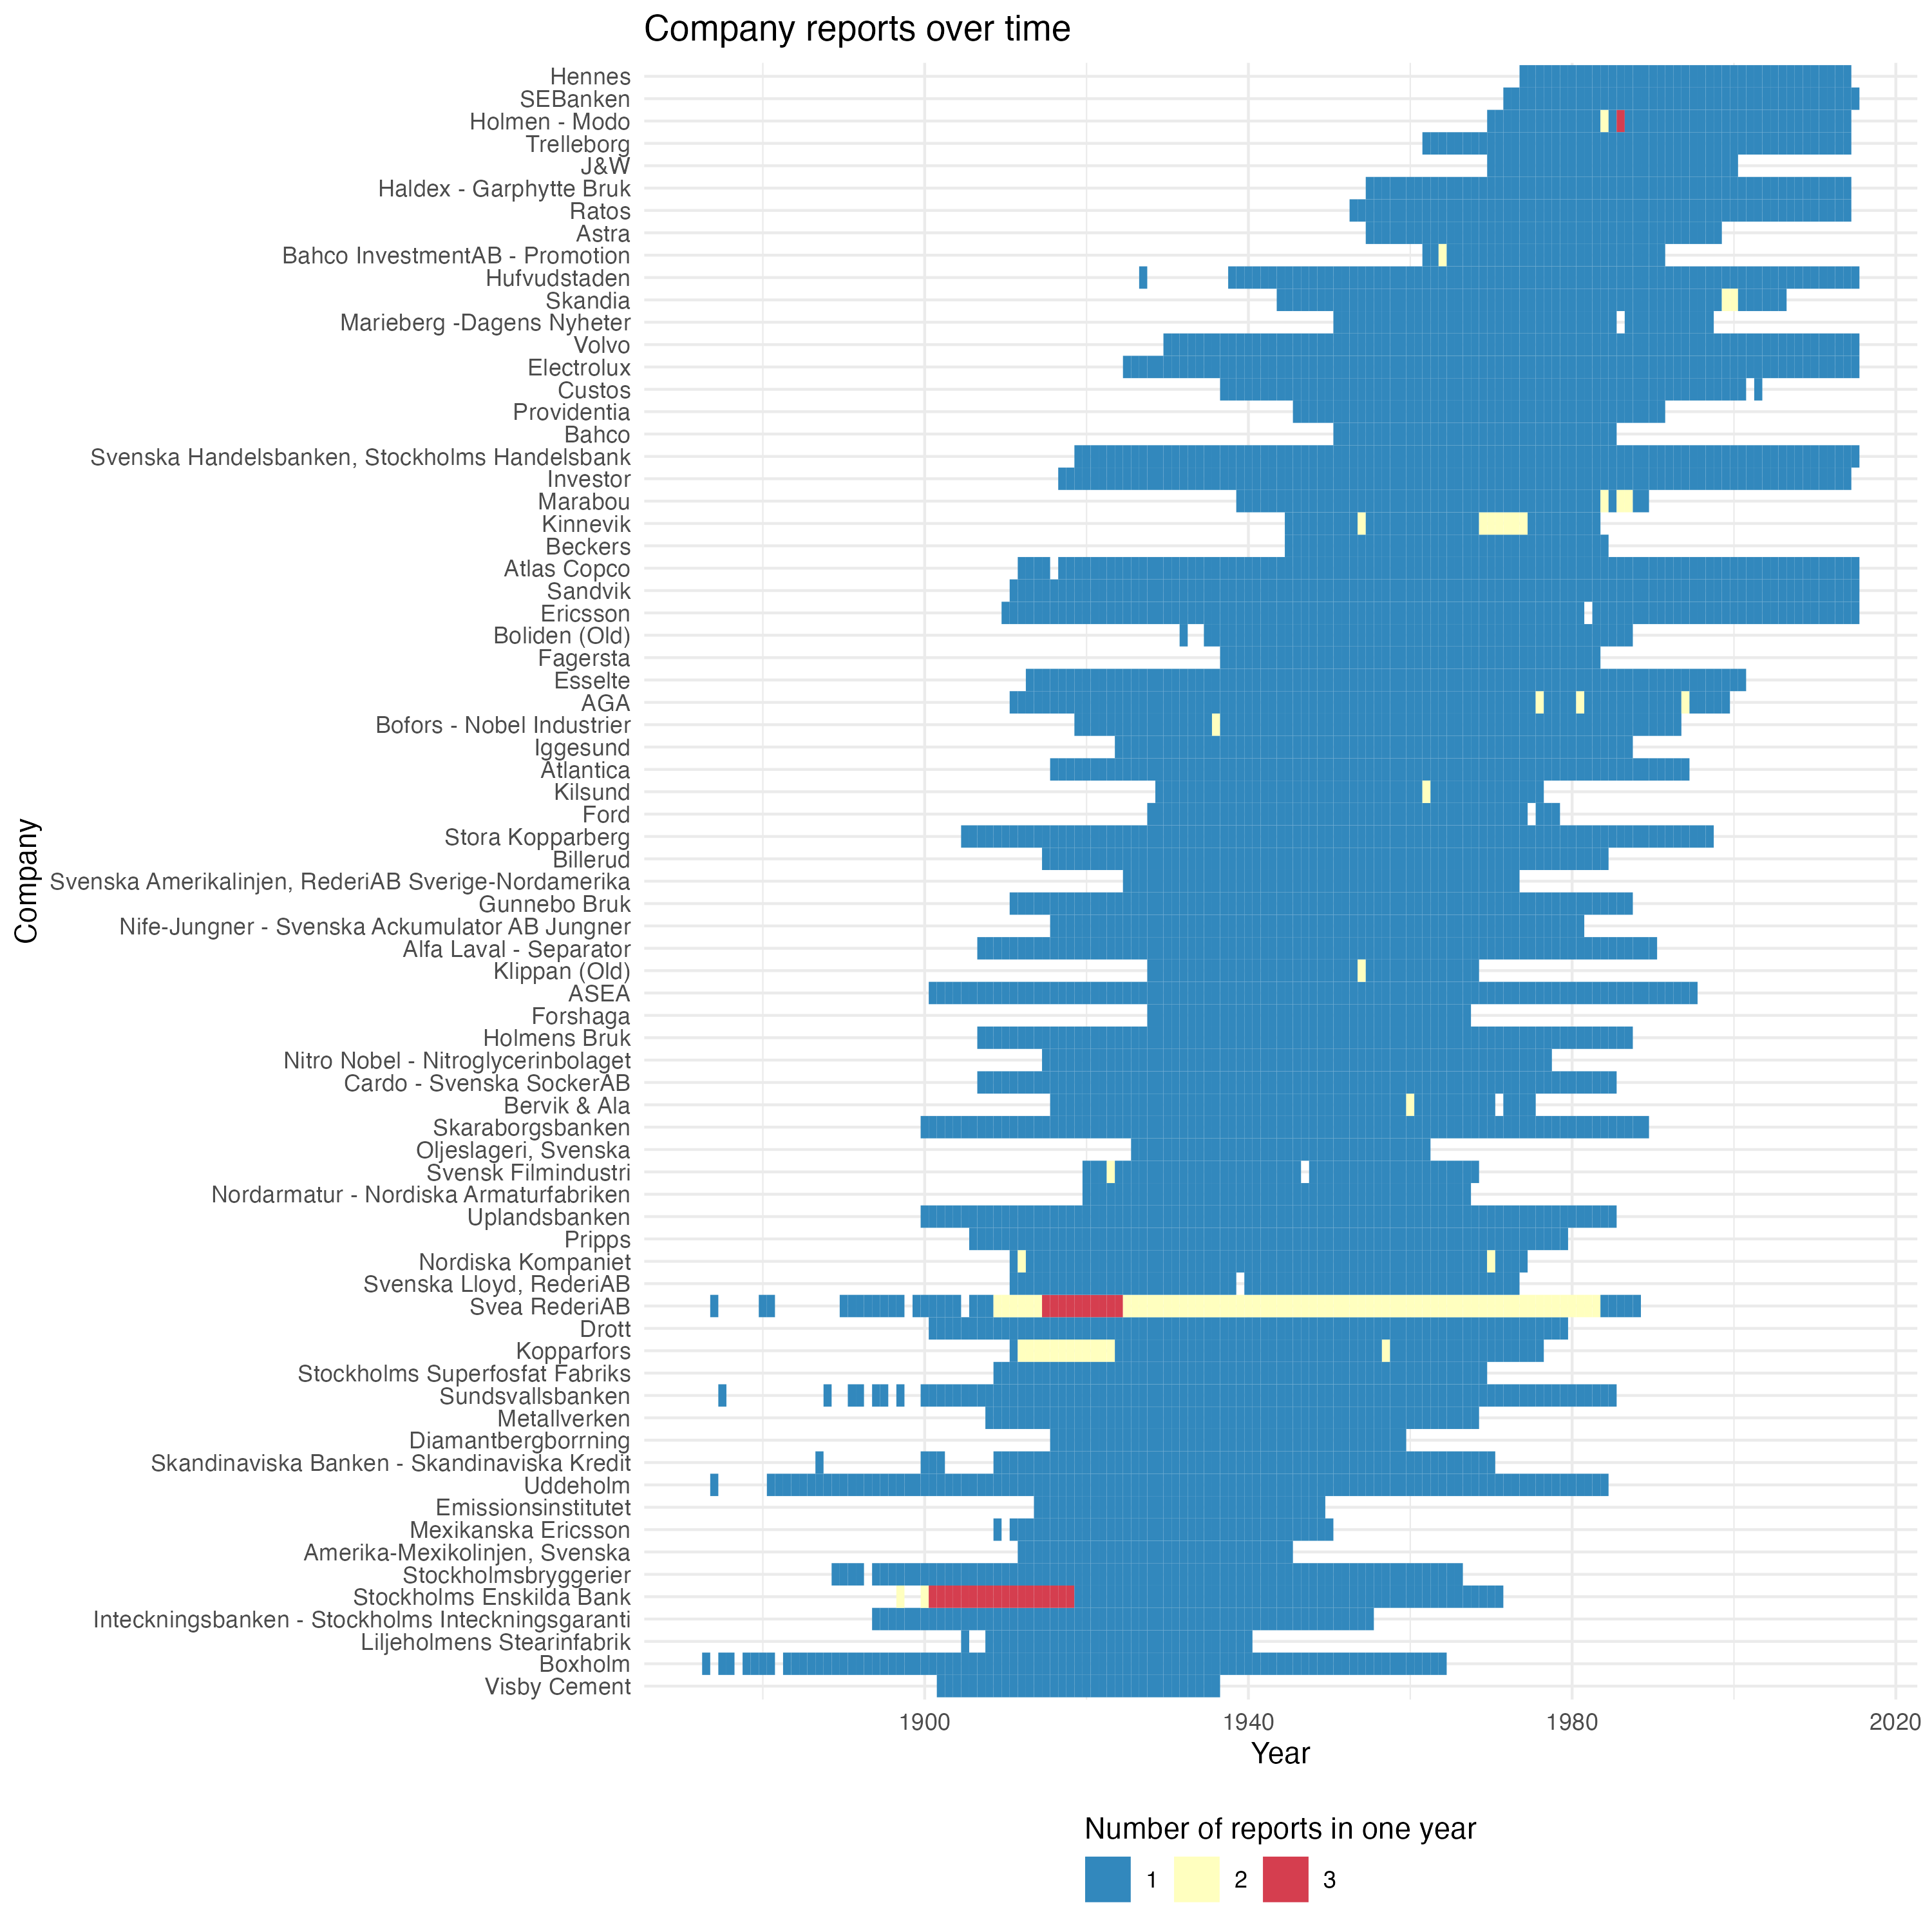
\includegraphics{images/company_reports_over_time.png}

}

\caption{\label{fig-crot}Annual Report Coverage}

\end{figure}%

To know about each director's educational background, international
experience, and broader career trajectory, information was gathered from
Swedish biographical dictionaries \emph{Vem är Vem?} and \emph{Vem är
Det?}. These references document education (e.g., engineering
vs.~business), overseas postings or study, and other notable career
milestones. I detail the digitization of this data in the third paper of
my thesis, and include a summary below.

\subsubsection{Data Collection and
Digitization}\label{data-collection-and-digitization}

The digitization process involved scraping the scanned archival annual
reports from the Stockholm School of Economics Library - which along
with drawing on their own archive, collected some reports from the Royal
Library and Centrum för Näringslivshistoria to fill coverage gaps. This
scraping script is available in the code repository linked above.

A novel digitization process was needed to manage changes in financial
reporting and layout over eight decades. Conventional Optical Character
Recognition (OCR) methods proved insufficient due to inconsistent table
structures, especially when reports extended over multiple pages to
detail subsidiaries and international branches. Instead, the project
used Large Language Models from Google's ``Gemini'' family, combined
with a custom pydantic data schema, to extract structured information
from images. This approach sidestepped the need for traditional OCR by
relying on multimodal image-processing capabilities, which improved
accuracy and consistency. Nonetheless, certain complexities remain.
Reporting language gradually shifted from Swedish to English for some
companies, and the scope of financial disclosure expanded, with some
early reports totaling only two pages and later ones exceeding one
hundred. Although the main income statement and balance sheet items
remained comparable, firm-level coverage of current assets, current
liabilities, and subsidiary performance varied from year to year. The
data is made accessible in the code repository linked above, as well as
in an
\href{https://swedish-annual-reports-archive-explorer.streamlit.app/}{interactive
dashboard for exploration}, detailed in Figure~\ref{fig-data-portal}.

Despite these technical advances, certain challenges remained.
Variations in balance sheet reporting posed difficulties, as some firms
presented multi-page breakdowns of assets or liabilities across
subsidiaries or international branches, making it difficult to aggregate
consistently. Additionally, language changes over time added complexity;
reporting language shifted from Swedish to English in the mid-20th
century for some companies. This issue was partially addressed by
prompting the extraction models to recognize both Swedish and English
terms, as evidenced in the reproduced PyDantic data schema in the
appendix.

\newpage{}

\begin{figure}

\begin{minipage}{0.50\linewidth}

\centering{

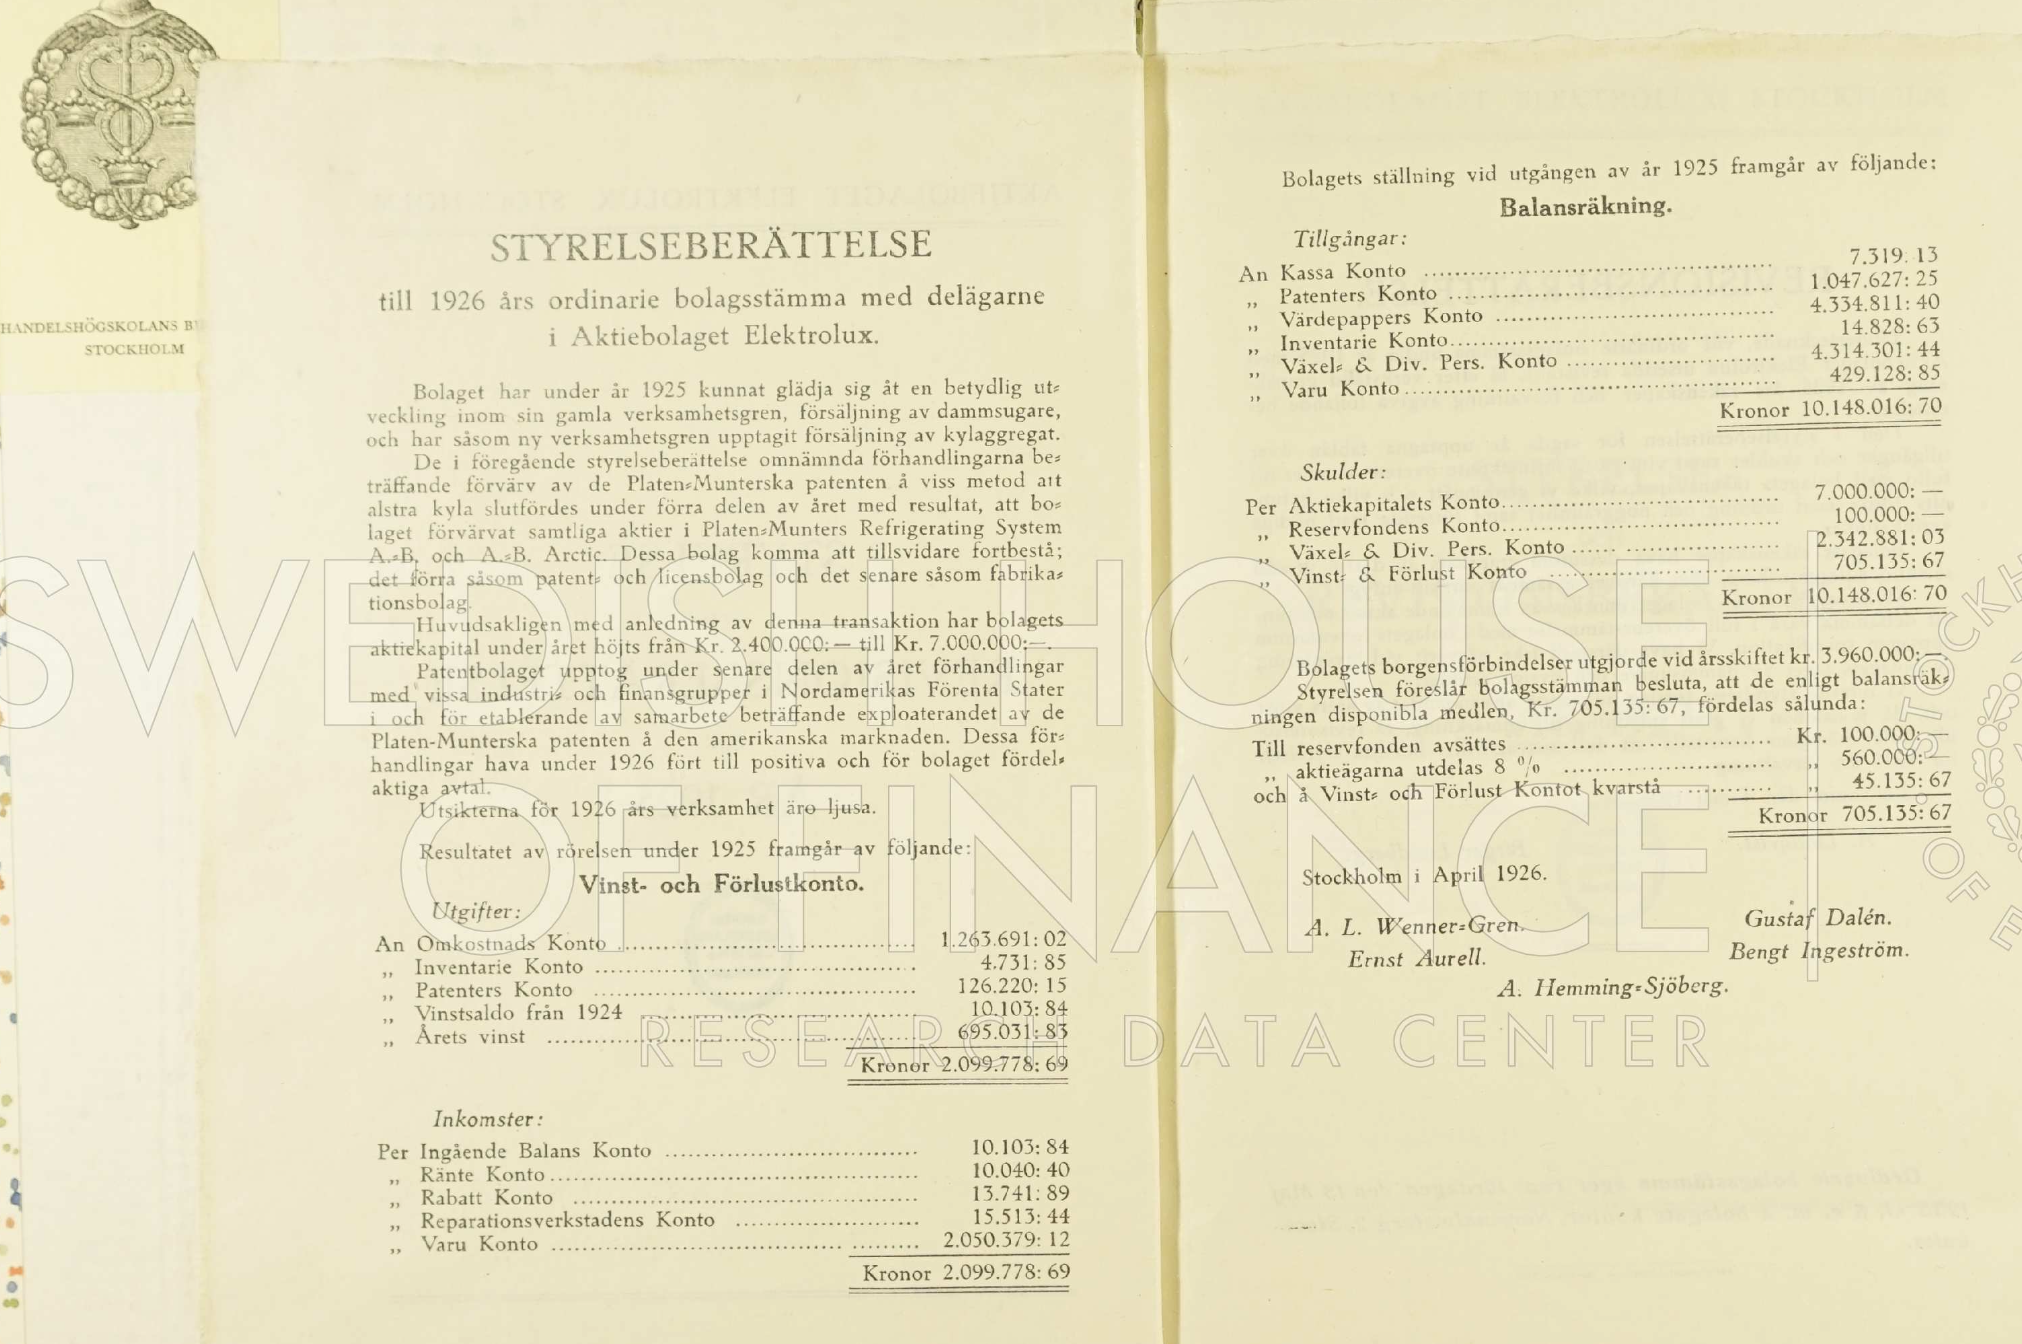
\includegraphics{images/report-1.png}

}

\subcaption{\label{fig-cri-1925}1925}

\end{minipage}%
%
\begin{minipage}{0.50\linewidth}

\centering{

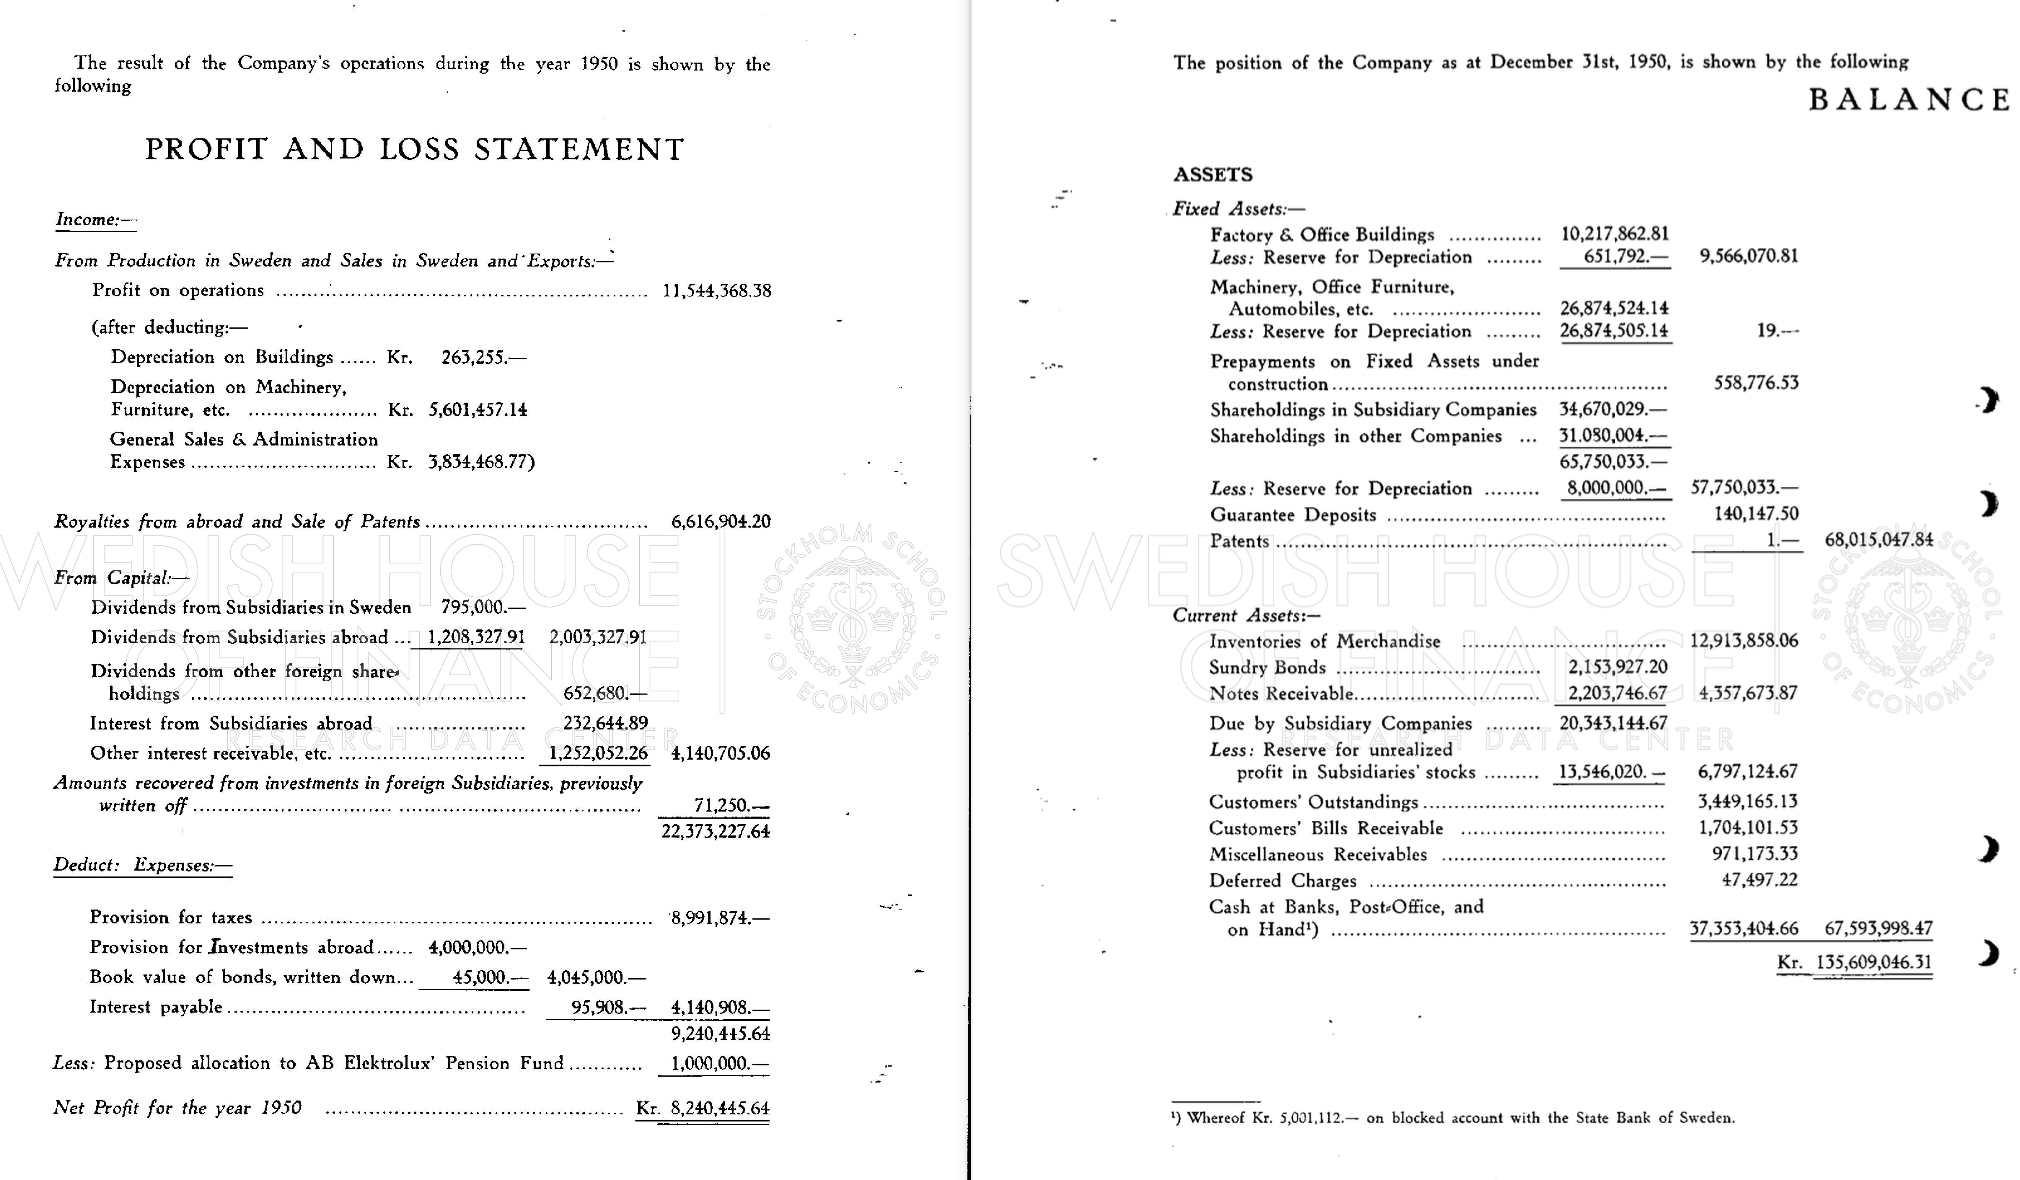
\includegraphics{images/report-2.png}

}

\subcaption{\label{fig-cri-1950}1950}

\end{minipage}%
\newline
\begin{minipage}{0.50\linewidth}

\centering{

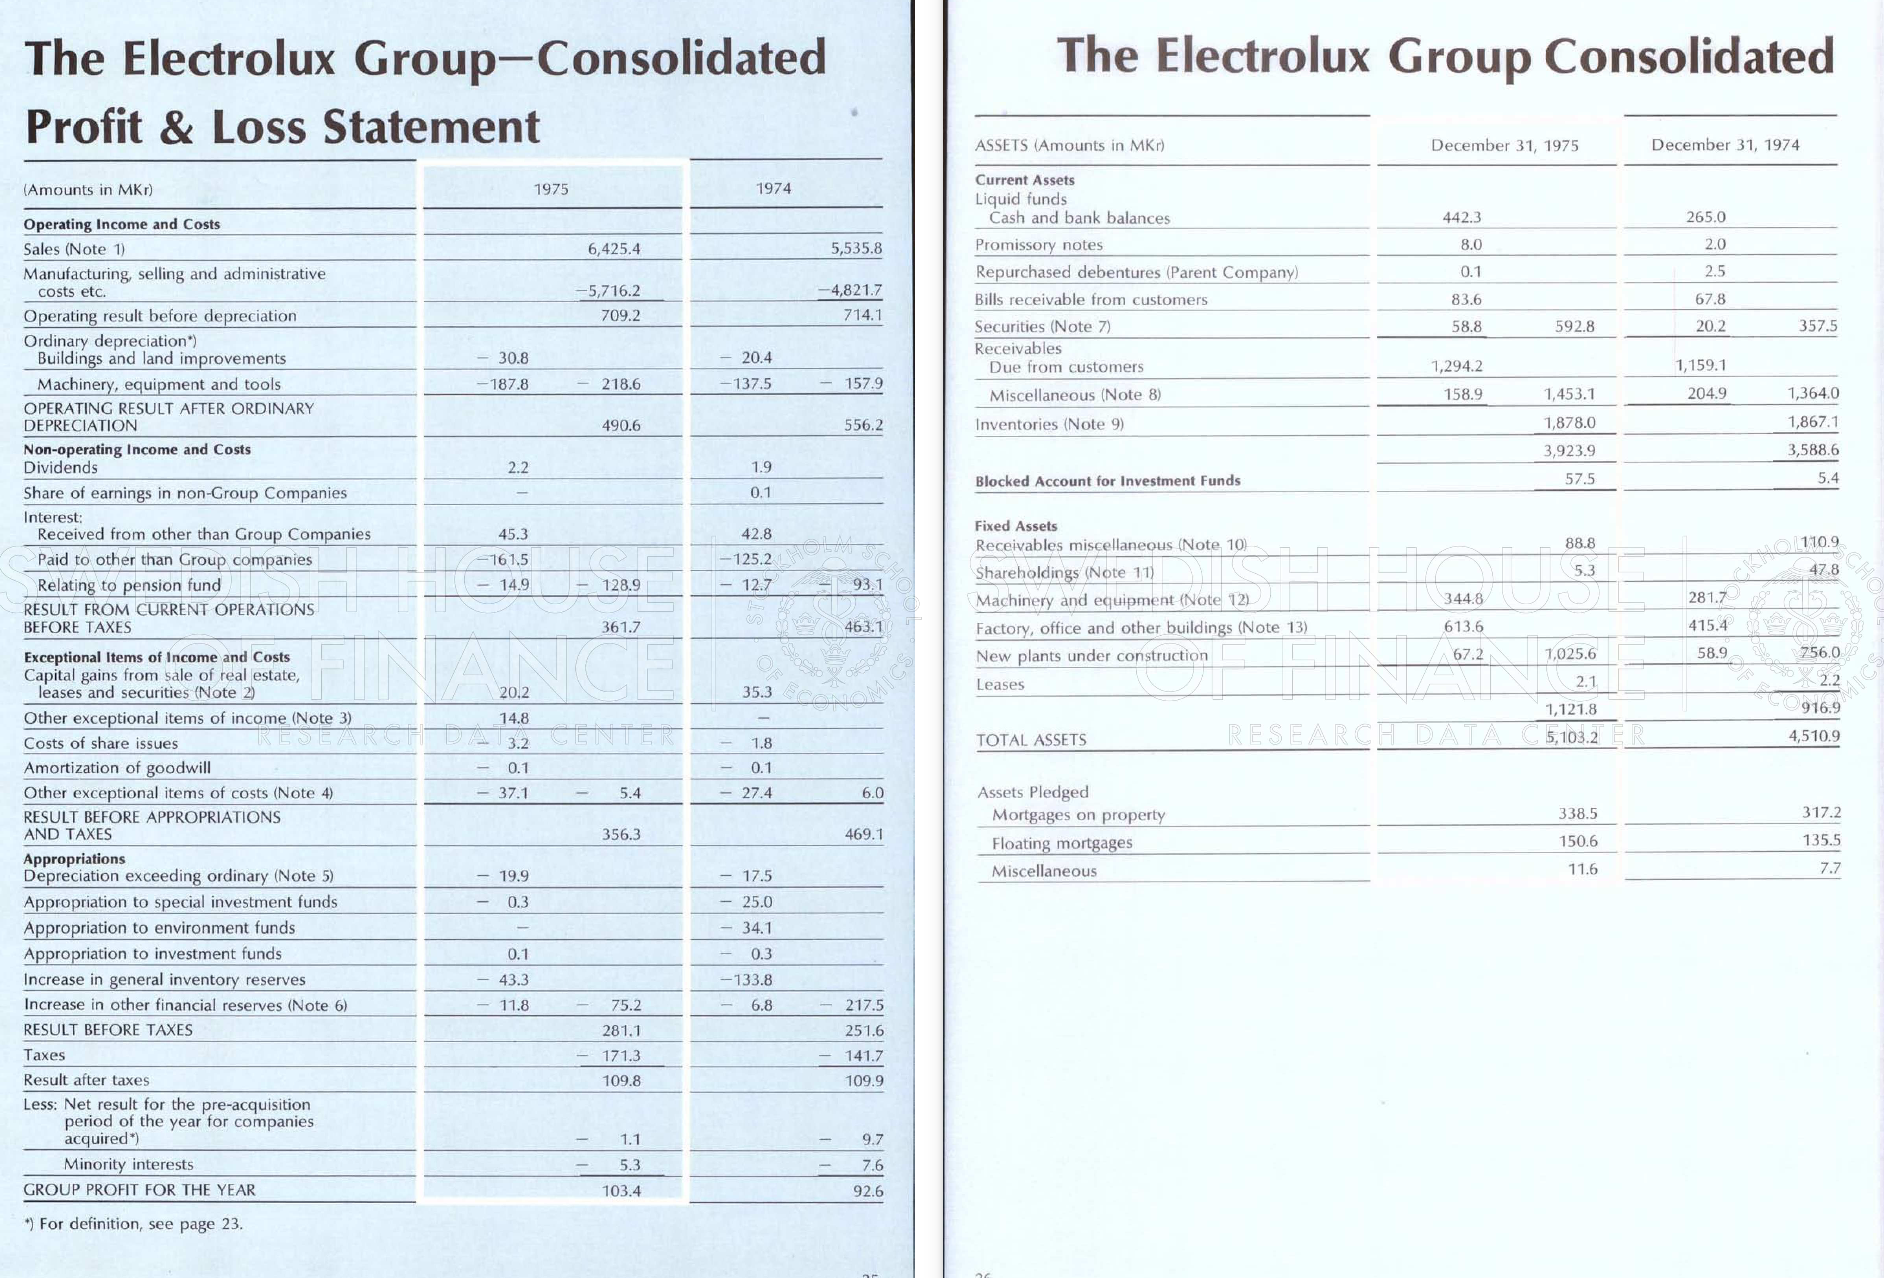
\includegraphics{images/report-3.png}

}

\subcaption{\label{fig-cri-1975}1975}

\end{minipage}%

\caption{\label{fig-reportsone}Profit and Loss Statements and Balalnce
Sheets for Electrolux AB from 1925, 1950, and 1975. Souce: Swedish House
of Finance at the Stockholm School of Economics Library Archives.}

\end{figure}%

\newpage{}

Board composition data were generally easier to extract, given that
names and positions typically appeared in a standard location beneath
the balance sheet. Individual directors' surnames, initials, full names,
and any listed title (e.g., Verkställande Direktör or Ordförande) were
recorded.

To supplement these board lists with directors' backgrounds, a fuzzy
string-matching algorithm was employed to match board members against
the \emph{Vem är Vem?} and \emph{Vem är Det?} biographical dictionaries.
Approximately 72\% of board members were successfully matched using
surname and initials; improving upon this match rate --- potentially by
incorporating mentions of employers or corporate affiliations into the
matching routine --- remains an area for future work. In the later
periods towards 1980, the match rate drops slightly as we are drawing
mainly on the \emph{Vem är Det?} biographical dictionaries, which are
published later and have less coverage than the \emph{Vem är Vem?}
volumes. It would be possible to improve the match rate by expanding the
search to other biographical dictionaries such as the SBL, or company
archives, but this is beyond the scope of the paper at present.

An example of the biographical data is shown in Figure~\ref{fig-vav-1},
and the distribution of biographies across volumes and time period is
shown in Figure~\ref{fig-vav-2}.

\subsubsection{Source Criticism}\label{source-criticism}

Although these biographical dictionaries offer a valuable repository of
career information, they have certain limitations. Inclusion was partly
self-selective, in that individuals could pay a nominal fee to appear,
and the depth of information varies from one entry to another. A
comparison with the Swedish Biographical Lexicon (SBL), which selects
figures on broader historical grounds, revealed that fewer than
one-fifth of the sampled individuals from Vem är Vem? also appear in the
SBL. This discrepancy implies that Vem är Vem? may overrepresent
socially prominent individuals, but that limitation is less
consequential for studying board members of listed firms, who tend to
hold influential positions by definition. Nonetheless, caution is
warranted when interpreting patterns of foreign training or professional
networking, since those who invested in a biographical listing may
differ systematically from peers who did not.

\begin{figure}

\begin{minipage}{0.50\linewidth}

\centering{

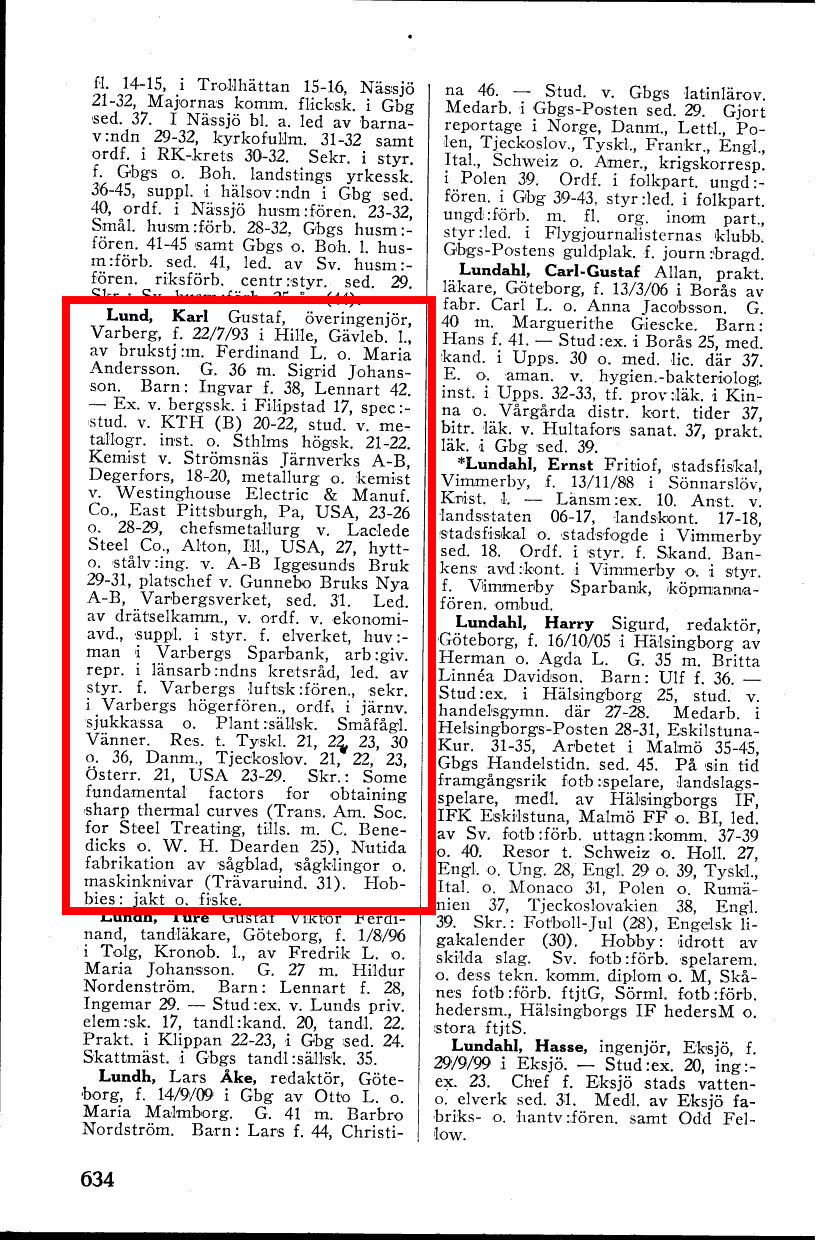
\includegraphics{images/vem_page-1.png}

}

\subcaption{\label{fig-vav-1}An example of a biogaphy from Karl Gustav
Lund}

\end{minipage}%
%
\begin{minipage}{0.50\linewidth}

\centering{

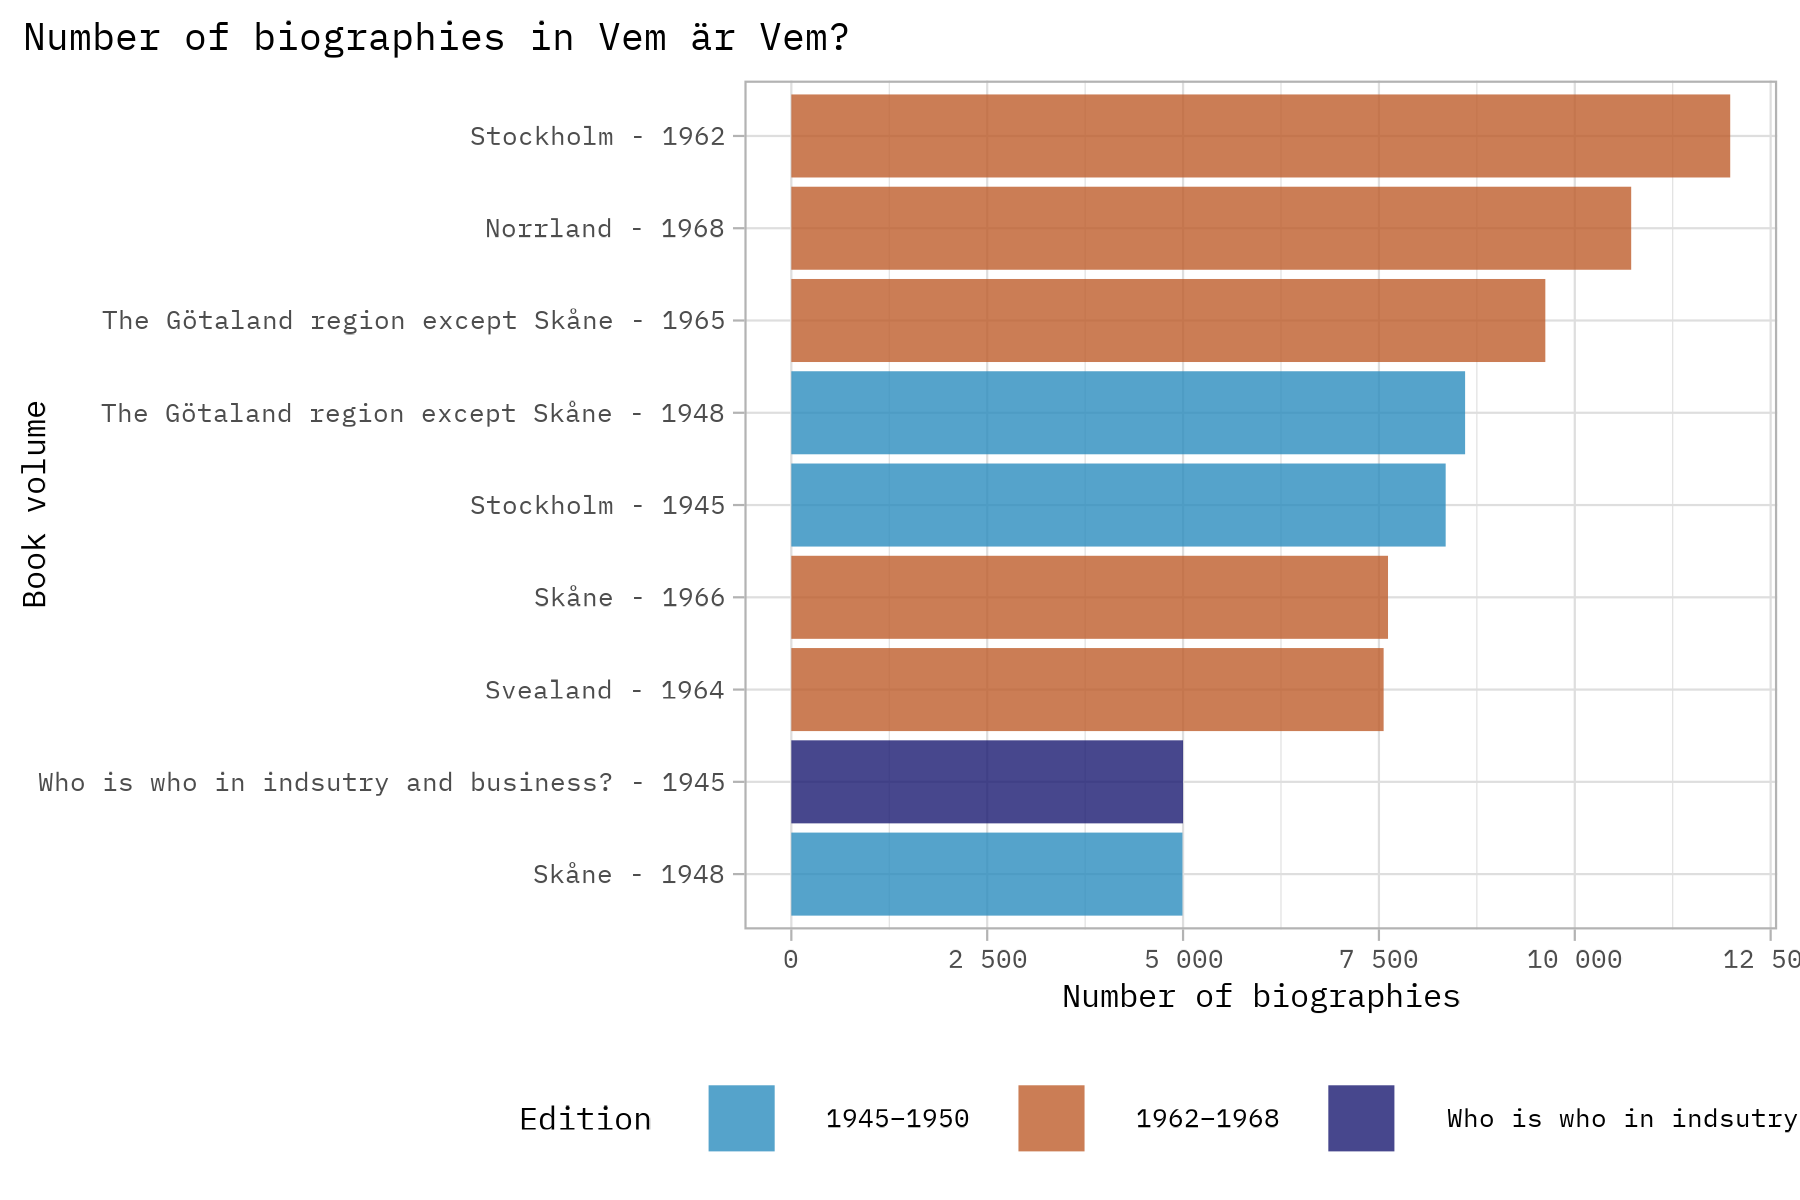
\includegraphics{images/who-is-who-volumes-2.png}

}

\subcaption{\label{fig-vav-2}Number of biographies in each volume of
`Vem är Vem?'}

\end{minipage}%

\caption{\label{fig-vemarvem}Example of a biographical entry from
\emph{Vem är Vem?} and the number of biographies in each volume. Source:
Projekt Runeberg scans of \emph{Vem är Vem?} volumes and author's own
analysis.}

\end{figure}%

Another key limitation involves the composition of the 71 firms under
study. The sample primarily includes the largest listed companies, many
of which are finance and investment entities or engineering and
industrial firms. According to internal categorization, finance and
investment comprises 30.43 percent of the sample and engineering and
industrial another 20.29 percent, with the remainder distributed across
consumer goods, mining and metals, telecommunications, technology,
automotive, and machinery. These proportions mean that the findings will
not necessarily generalize to smaller, non-listed firms in other
sectors. See Table~\ref{tbl-industry-distribution} for a breakdown of
the sample by broad industry classification.

\begin{longtable}[]{@{}ll@{}}
\caption{Distribution of firms in sample by broad industry
classification.}\label{tbl-industry-distribution}\tabularnewline
\toprule\noalign{}
Broad Industry & Percentage (\%) \\
\midrule\noalign{}
\endfirsthead
\toprule\noalign{}
Broad Industry & Percentage (\%) \\
\midrule\noalign{}
\endhead
\bottomrule\noalign{}
\endlastfoot
Finance \& Investment & 30.43\% \\
Engineering \& Industrial & 20.29\% \\
Other & 18.84\% \\
Consumer Goods & 15.94\% \\
Mining \& Metals & 7.25\% \\
Telecommunications \& Technology & 4.35\% \\
Automotive \& Machinery & 2.90\% \\
\end{longtable}

\subsubsection{Constructing Variables}\label{constructing-variables}

Firm coverage being such as it is, I then construct several key
variables to test whether boards with engineers that have experience in
the United States performed differently. The first variable is the
presence of a board member who has documented work experience in the
United States. This information is extracted from the biographical
dictionaries, which often note foreign postings or study abroad. I
differentiate between individuals who travel to foreign counties,
another commonly listed attribute in the biographical dictionaries, and
individuals who work overseas by requiring the name of a firm that an
individual worked at abroad to be present.

Regarding board composition, this is coded both in binary form -
indicating that at least one such individual exists - or by a share with
the number of U.S.-trained engineers on the board. I use both
specifications in the analysis.

Additional categorization sorts directors by educational background
(e.g., engineering versus business), based on their educational degree
and institute, if available. These classifications, drawn from
dictionary entries, can show the relative importance of foreign exposure
in shaping corporate practices.

The outcome measures center on firm performance, particularly revenue
per employee and net revenue. Revenue per employee is especially useful
for analyzing potential productivity gains or labor-saving measures.

Regarding networks, a bipartite network of firms and directors is
created in order to provide variables to the time series analysis. A
bipartite network has two kinds of nodes. On the one side, there are
board members who can serve on different boards, and on the other, are
firms which are connected by common board members. Such a network allows
me to measure whether strongly interconnected firms exhibit similar
policy decisions, employment trends, or performance trajectories.
Standard measures of centrality - degree, betweenness, or eigenvector -
are used to test whether firms situated in well-connected networks share
similar characteristics or outcomes.

Overall, the dataset assembled here---covering both extensive financial
records and board composition details---enables an investigation of how
U.S.-experienced engineers affected firm productivity and employment
strategies in twentieth-century Sweden. While the archival approach and
the reliance on biographical dictionaries introduce certain biases, the
consistency of key income statement and balance sheet items, combined
with the strength of the board-level matching, provides a valuable
foundation for analyzing historical corporate governance.

\subsection{IV. Empirical Method}\label{iv.-empirical-method-1}

The empirical analysis begins with a longitudinal design that exploits
firm-level data assembled from 1873 to 1980. Each firm enters the panel
in years where sufficient financial information and board composition
records exist, forming an unbalanced panel that covers varying intervals
for different companies, where coverage is shown in
Figure~\ref{fig-crot}. This approach allows for the exploration of how
changes within each firm---such as the arrival of a U.S.-experienced
engineer on the board---correlate with shifts in its performance
indicators. By including firm fixed effects, the regression
specifications control for any unobserved, time-invariant
characteristics of individual companies, such as historical reputations,
founding conditions, or long-standing ownership structures. Time
dummies, capturing broad economic cycles and periods of expansion or
downturn, help further isolate the relationship between board
composition and performance from macroeconomic influences.

The primary outcome variable is revenue per employee, chosen to
approximate labor productivity. This measure is constructed by dividing
a company's reported revenues by its total number of employees for each
year. Using revenue per employee helps detect whether board-level
decisions, including technological investments or operational
strategies, are associated with measurable gains in productivity. The
key explanatory variables focus on the presence and proportion of
directors with specialized backgrounds. One specification includes a
binary indicator that equals one if any board member meets two criteria:
holding an engineering education and having worked in the United States.
A complementary specification substitutes this binary measure with a
continuous one, reflecting the share of board members who fit the same
criteria. To address the sub-question about contrasting the effects of
business- or finance-trained directors, further terms partition board
composition into two dimensions: first, whether a director has an
engineering or business/finance background, and second, whether that
individual has foreign experience in the United States. In practice,
this is done by interacting the director's training (engineer
vs.~business/finance) with the U.S.-experience indicator, allowing the
regression coefficients to capture how these backgrounds combine in
shaping performance.

The estimated model includes the fundamental controls that appear in
most firm-level empirical studies of historical corporate governance.
Firm size enters, typically as the logarithm of total assets or
employment, to capture economies of scale and general capacity for
investment. Firm age, constructed from the date of incorporation or
earliest available archival record, accounts for the possibility that
older firms have distinct trajectories for performance or governance
structures. Industry composition is controlled through sector dummies
based on the classification in table
Table~\ref{tbl-industry-distribution}, where each firm is assigned to
one of several categories---such as finance and investment, engineering
and industrial, or consumer goods---thereby helping to account for the
varying technological demands or competitive pressures across different
types of enterprises. Time effects are managed by incorporating year
fixed effects or, when data permit, a set of time-period dummies to
smooth out fluctuations tied to global economic shocks, wars, or postwar
recoveries.

Though revenue per employee is the preferred measure of firm
performance, a similar regression can be run where total employment or
employment growth becomes the dependent variable. If new board
appointments encourage expansion, the results may appear as higher labor
uptake over time, especially if technological innovations initially
require more specialized engineers or skilled staff. Alternatively, if
the emphasis of U.S.-trained engineers falls on productivity
improvements rather than labor growth, the parameter estimates for
employment would remain modest while revenue per employee rises.
Comparing both sets of equations allows a fuller assessment of whether
board composition shapes only productivity or also influences hiring
decisions.

Taken together, this panel regression framework aims to detect whether
directors' backgrounds---particularly those with engineering expertise
and foreign experience---are systematically tied to firm outcomes beyond
mere chance associations. By combining firm fixed effects, a wide span
of time, and a set of relevant controls, the analysis seeks to
distinguish patterns that emerge when new expertise is introduced or
lost at the board level, providing insights into the ways that technical
and international knowledge may have steered corporate strategies toward
higher productivity in Swedish industry.

The specification is:

{[} \text{Let } i \text{ index firms and } t
\text{ index years. The preferred empirical specification for the panel analysis of revenue per employee can be written as:}
{]}

{[} \text{RevenuePerEmployee}\emph{\{i,t\} = \alpha +
\beta}\{1\},(\text{ShareUSExpEngineers})\emph{\{i,t\} +
\beta}\{2\},(\text{Controls})\emph{\{i,t\} + \gamma}\{i\} +
\delta\emph{\{t\} + \varepsilon}\{i,t\}. {]}

In this specification, \(\text{RevenuePerEmployee}_{i,t}\) is the
primary outcome variable, measuring the firm's total sales divided by
its number of employees. The explanatory term
\((\text{ShareUSExpEngineers})_{i,t}\) is the proportion of board
members in firm \(i\) and year \(t\) who combine an engineering
background with documented work experience in the United States. This
variable may capture how technology-focused expertise, supplemented by
exposure to American industrial or managerial practices, shapes
productivity outcomes.

The vector \((\text{Controls})_{i,t}\) includes relevant firm-level
characteristics, such as logarithm of total assets, firm age, and sector
indicators drawn from table \(\text{@tbl-industry-distribution}\).
Including these controls accounts for the possibility that older or
larger firms, or certain industrial classifications, systematically
differ in how effectively they convert workforce inputs into revenue. In
addition, macroeconomic or temporal shifts are addressed by
\(\delta_{t}\), a year fixed effect that nets out time-specific shocks
such as recessions or wartime disruptions. Meanwhile, \(\gamma_{i}\) is
a firm fixed effect that absorbs all time-invariant attributes of each
company, such as founding conditions, enduring ownership patterns, or
longstanding reputations.

Finally, \(\varepsilon_{i,t}\) is the idiosyncratic error term. Standard
errors in such models are typically clustered by firm to allow for
heteroskedasticity and serial correlation within each company's
observations. This framework is designed to disentangle how board
composition---particularly the presence and share of U.S.-experienced
engineers---relates to productivity measures like revenue per employee,
while holding constant all other observable and unobservable differences
among firms across the historical period under study.

\newpage{}

\subsection{Appendix}\label{appendix}

\paragraph{List of Companies in the
Dataset}\label{list-of-companies-in-the-dataset}

\begin{longtable}[]{@{}
  >{\raggedright\arraybackslash}p{(\columnwidth - 2\tabcolsep) * \real{0.3056}}
  >{\raggedright\arraybackslash}p{(\columnwidth - 2\tabcolsep) * \real{0.6944}}@{}}
\toprule\noalign{}
\begin{minipage}[b]{\linewidth}\raggedright
Company Name
\end{minipage} & \begin{minipage}[b]{\linewidth}\raggedright
Classification/Industry
\end{minipage} \\
\midrule\noalign{}
\endhead
\bottomrule\noalign{}
\endlastfoot
AGA & Industrial gases \& chemical technology \\
ASEA & Electrical engineering \& industrial technology \\
Addo & Office machines \& calculators \\
AlfortCronholm & Wholesale trade (hardware and tools) \\
Arvikaverken & Heavy machinery / industrial engineering \\
Astra & Pharmaceuticals \& healthcare \\
Atlantica & Insurance services \\
Bahco & Hand tools \& metalworking equipment \\
Baltic & Shipping / maritime services \\
Beckers & Paints \& coatings \\
Beijerinvest & Investment \& holding company \\
Billerud & Pulp, paper \& packaging \\
Billman & Engineering components (industrial valves) \\
Boxholm & Steel production \& metal fabrication \\
Coronaverken & Iron \& steel works \\
Custos & Investment \& holding company \\
Diamantbergborrning & Mining \& drilling (mining services) \\
Diligentia & Real estate \& property management \\
Drott & Real estate \& property management \\
Electrolux & Home appliances \& consumer electronics \\
Emissionsinstitutet & Environmental research \& consultancy \\
Ericsson & Telecommunications \& networking equipment \\
Esselte & Office products \& stationery \\
Exportinvest & Investment \& export finance \\
Fagersta & Steel \& metallurgical engineering \\
Fannyudde & Engineering \& manufacturing (marine equipment) \\
Ford & Automotive manufacturing (Swedish operations) \\
Forshaga & Chemical industry (plastics and resins) \\
Heimdall & Security services \\
Hennes & Fashion retail (origin of H\&M) \\
Hufvudstaden & Real estate \& property management \\
Iggesund & Iron \& steel, later pulp and paper \\
Incentive & Investment \& holding company \\
Investor & Investment \& holding company \\
Invik & Investment \& finance \\
JW & Engineering \& manufacturing (industrial equipment) \\
Kilsund & Maritime engineering \& metal works \\
Kinnevik & Investment \& holding company \\
Kopparfors & Forestry \& paper industry \\
Kreditbanken & Banking \& finance \\
Lux & Consumer goods (lighting/appliances) \\
Marabou & Confectionery \& food production \\
Metallverken & Metalworking \& industrial manufacturing \\
Neptun & Maritime services (tugboats and salvage) \\
Nessim & Investment \& finance \\
Nordbanken & Banking \& finance \\
Norrlandsbanken & Banking \& finance \\
Optimus & Portable stoves \& heating equipment \\
PLM & Packaging \& containers \\
Papyrus & Stationery \& paper products \\
Pripps & Brewery \& beverage production \\
Providentia & Investment \& holding company \\
Pumpseparator & Industrial equipment (fluid handling) \\
Ratos & Investment \& holding company \\
SEBanken & Banking \& finance \\
Sandvik & Engineering (materials technology \& mining tools) \\
Skandia & Insurance \& financial services \\
Skaraborgsbanken & Banking \& finance \\
Sonesson & Consumer goods (food production) \\
Stockholmsbryggerier & Brewery \& beverage production \\
Sulitelma & Mining (zinc and copper) \\
Sundsvallsbanken & Banking \& finance \\
Tarkett & Flooring \& building materials \\
Tjenstemannabanken & Banking \& finance (service bank) \\
Trelleborg & Industrial engineering (polymer-based products) \\
Uddeholm & Tool steels \& metallurgical production \\
Uplandsbanken & Banking \& finance \\
Volta & Electrical appliances (vacuum cleaners) \\
Volvo & Automotive \& heavy machinery manufacturing \\
\end{longtable}

\paragraph{Summary of companies}\label{summary-of-companies}

\begin{longtable}[]{@{}ll@{}}
\toprule\noalign{}
Broad Industry & Percentage (\%) \\
\midrule\noalign{}
\endhead
\bottomrule\noalign{}
\endlastfoot
Finance \& Investment & 30.43\% \\
Engineering \& Industrial & 20.29\% \\
Other & 18.84\% \\
Consumer Goods & 15.94\% \\
Mining \& Metals & 7.25\% \\
Telecommunications \& Technology & 4.35\% \\
Automotive \& Machinery & 2.90\% \\
\end{longtable}

\newpage{}

\begin{Shaded}
\begin{Highlighting}[]
\CommentTok{\# {-}{-}{-} Pydantic Models {-}{-}{-}}

\KeywordTok{class}\NormalTok{ IncomeStatement(BaseModel):}
    \CommentTok{"""}
\CommentTok{    Standard representation of an Income Statement.}
\CommentTok{    Note: In many older reports, board member names are listed below this statement.}
\CommentTok{    """}
\NormalTok{    revenue: Optional[}\BuiltInTok{float}\NormalTok{] }\OperatorTok{=}\NormalTok{ Field(}
        \VariableTok{None}\NormalTok{, description}\OperatorTok{=}\StringTok{"Total revenues or sales. (Swedish: Intäkter)"}
\NormalTok{    )}
\NormalTok{    cost\_of\_goods\_sold: Optional[}\BuiltInTok{float}\NormalTok{] }\OperatorTok{=}\NormalTok{ Field(}
        \VariableTok{None}\NormalTok{, description}\OperatorTok{=}\StringTok{"Cost of goods sold. (Swedish: Kostnad såld vara)"}
\NormalTok{    )}
\NormalTok{    operating\_expenses: Optional[}\BuiltInTok{float}\NormalTok{] }\OperatorTok{=}\NormalTok{ Field(}
        \VariableTok{None}\NormalTok{, description}\OperatorTok{=}\StringTok{"Total operating expenses. (Swedish: Rörelsekostnader)"}
\NormalTok{    )}
\NormalTok{    wages\_expense: Optional[}\BuiltInTok{float}\NormalTok{] }\OperatorTok{=}\NormalTok{ Field(}
        \VariableTok{None}\NormalTok{, description}\OperatorTok{=}\StringTok{"Total wages and salaries expense. (Swedish: Lönekostnader)"}
\NormalTok{    )}
\NormalTok{    tax\_expense: Optional[}\BuiltInTok{float}\NormalTok{] }\OperatorTok{=}\NormalTok{ Field(}\VariableTok{None}\NormalTok{, description}\OperatorTok{=}\StringTok{"Tax expense. (Swedish: Skatt)"}\NormalTok{)}
\NormalTok{    depreciation: Optional[}\BuiltInTok{float}\NormalTok{] }\OperatorTok{=}\NormalTok{ Field(}\VariableTok{None}\NormalTok{, description}\OperatorTok{=}\StringTok{"Depreciation (Swedish: Avskrivningar)"}\NormalTok{)}
\NormalTok{    net\_income: Optional[}\BuiltInTok{float}\NormalTok{] }\OperatorTok{=}\NormalTok{ Field(}
        \VariableTok{None}\NormalTok{, description}\OperatorTok{=}\StringTok{"Net income (profit or loss) for the period. (Swedish: Årets resultat)"}
\NormalTok{    )}


\KeywordTok{class}\NormalTok{ BalanceSheet(BaseModel):}
    \CommentTok{"""}
\CommentTok{    Standard representation of a Balance Sheet.}
\CommentTok{    """}
\NormalTok{    total\_assets: Optional[}\BuiltInTok{float}\NormalTok{] }\OperatorTok{=}\NormalTok{ Field(}
        \VariableTok{None}\NormalTok{, description}\OperatorTok{=}\StringTok{"Total assets at period end. (Swedish: Tillgångar)"}
\NormalTok{    )}
\NormalTok{    current\_assets: Optional[}\BuiltInTok{float}\NormalTok{] }\OperatorTok{=}\NormalTok{ Field(}
        \VariableTok{None}\NormalTok{, description}\OperatorTok{=}\StringTok{"Current assets. (Swedish: Omsättningstillgångar)"}
\NormalTok{    )}
\NormalTok{    fixed\_assets: Optional[}\BuiltInTok{float}\NormalTok{] }\OperatorTok{=}\NormalTok{ Field(}
        \VariableTok{None}\NormalTok{, description}\OperatorTok{=}\StringTok{"Long{-}term or fixed assets. (Swedish: Anläggningstillgångar)"}
\NormalTok{    )}
\NormalTok{    total\_liabilities: Optional[}\BuiltInTok{float}\NormalTok{] }\OperatorTok{=}\NormalTok{ Field(}
        \VariableTok{None}\NormalTok{, description}\OperatorTok{=}\StringTok{"Total liabilities. (Swedish: Skulder)"}
\NormalTok{    )}
\NormalTok{    current\_liabilities: Optional[}\BuiltInTok{float}\NormalTok{] }\OperatorTok{=}\NormalTok{ Field(}
        \VariableTok{None}\NormalTok{, description}\OperatorTok{=}\StringTok{"Current liabilities. (Swedish: Kortfristiga skulder)"}
\NormalTok{    )}
\NormalTok{    long\_term\_liabilities: Optional[}\BuiltInTok{float}\NormalTok{] }\OperatorTok{=}\NormalTok{ Field(}
        \VariableTok{None}\NormalTok{, description}\OperatorTok{=}\StringTok{"Long{-}term liabilities. (Swedish: Långfristiga skulder)"}
\NormalTok{    )}
\NormalTok{    shareholders\_equity: Optional[}\BuiltInTok{float}\NormalTok{] }\OperatorTok{=}\NormalTok{ Field(}
        \VariableTok{None}\NormalTok{, description}\OperatorTok{=}\StringTok{"Total shareholders\textquotesingle{} or owners\textquotesingle{} equity. (Swedish: Eget kapital)"}
\NormalTok{    )}


\KeywordTok{class}\NormalTok{ BoardMember(BaseModel):}
    \CommentTok{"""}
\CommentTok{    Representation of a single board member.}
\CommentTok{    Typically listed below the Income Statement in older reports.}
\CommentTok{    """}
\NormalTok{    surname: }\BuiltInTok{str} \OperatorTok{=}\NormalTok{ Field(..., description}\OperatorTok{=}\StringTok{"The surname of the board member."}\NormalTok{)}
\NormalTok{    first\_name: Optional[}\BuiltInTok{str}\NormalTok{] }\OperatorTok{=}\NormalTok{ Field(}\VariableTok{None}\NormalTok{, description}\OperatorTok{=}\StringTok{"The first name of the board member."}\NormalTok{)}
\NormalTok{    initials: Optional[}\BuiltInTok{str}\NormalTok{] }\OperatorTok{=}\NormalTok{ Field(}\VariableTok{None}\NormalTok{, description}\OperatorTok{=}\StringTok{"Initials of the board member."}\NormalTok{)}
\NormalTok{    position: Optional[}\BuiltInTok{str}\NormalTok{] }\OperatorTok{=}\NormalTok{ Field(}\VariableTok{None}\NormalTok{, description}\OperatorTok{=}\StringTok{"The board position held by the member."}\NormalTok{)}


\KeywordTok{class}\NormalTok{ Auditor(BaseModel):}
    \CommentTok{"""}
\CommentTok{    Representation of a single auditor.}
\CommentTok{    Typically listed after the board members.}
\CommentTok{    """}
\NormalTok{    surname: }\BuiltInTok{str} \OperatorTok{=}\NormalTok{ Field(..., description}\OperatorTok{=}\StringTok{"The surname of the auditor."}\NormalTok{)}
\NormalTok{    first\_name: Optional[}\BuiltInTok{str}\NormalTok{] }\OperatorTok{=}\NormalTok{ Field(}\VariableTok{None}\NormalTok{, description}\OperatorTok{=}\StringTok{"The first name of the auditor."}\NormalTok{)}
\NormalTok{    initials: Optional[}\BuiltInTok{str}\NormalTok{] }\OperatorTok{=}\NormalTok{ Field(}\VariableTok{None}\NormalTok{, description}\OperatorTok{=}\StringTok{"Initials of the auditor."}\NormalTok{)}
\NormalTok{    auditing\_firm: Optional[}\BuiltInTok{str}\NormalTok{] }\OperatorTok{=}\NormalTok{ Field(}\VariableTok{None}\NormalTok{, description}\OperatorTok{=}\StringTok{"The auditing firm, if specified."}\NormalTok{)}


\KeywordTok{class}\NormalTok{ Employees(BaseModel):}
    \CommentTok{"""}
\CommentTok{    Representation of the number of employees in a company.}
\CommentTok{    """}
\NormalTok{    n\_employees: Optional[}\BuiltInTok{int}\NormalTok{] }\OperatorTok{=}\NormalTok{ Field(}\VariableTok{None}\NormalTok{, description}\OperatorTok{=}\StringTok{"Total number of employees. (Swedish: Antal anställda)"}\NormalTok{)}
\NormalTok{    n\_blue\_collar\_workers: Optional[}\BuiltInTok{int}\NormalTok{] }\OperatorTok{=}\NormalTok{ Field(}\VariableTok{None}\NormalTok{, description}\OperatorTok{=}\StringTok{"Total number of blue collar workers. (Swedish: Antal arbetare)"}\NormalTok{)}
\NormalTok{    n\_white\_collar\_workers: Optional[}\BuiltInTok{int}\NormalTok{] }\OperatorTok{=}\NormalTok{ Field(}\VariableTok{None}\NormalTok{, description}\OperatorTok{=}\StringTok{"Total number of white collar workers. (Swedish: Antal tjänstemän)"}\NormalTok{)}


\KeywordTok{class}\NormalTok{ FinancialReport(BaseModel):}
    \CommentTok{"""}
\CommentTok{    Comprehensive financial report model, including:}
\CommentTok{    {-} Income Statement (with Swedish term references)}
\CommentTok{    {-} Balance Sheet (with Swedish term references)}
\CommentTok{    {-} Employees (with Swedish term references)}
\CommentTok{    {-} Board members (often listed under the P\&L statement)}
\CommentTok{    {-} Auditors (often follow after the board list)}
\CommentTok{    """}
\NormalTok{    company\_name: }\BuiltInTok{str} \OperatorTok{=}\NormalTok{ Field(..., description}\OperatorTok{=}\StringTok{"The name of the company."}\NormalTok{)}
\NormalTok{    fiscal\_year: }\BuiltInTok{int} \OperatorTok{=}\NormalTok{ Field(..., description}\OperatorTok{=}\StringTok{"Fiscal year of the report."}\NormalTok{)}
\NormalTok{    income\_statement: IncomeStatement }\OperatorTok{=}\NormalTok{ Field(..., description}\OperatorTok{=}\StringTok{"Income statement details."}\NormalTok{)}
\NormalTok{    balance\_sheet: BalanceSheet }\OperatorTok{=}\NormalTok{ Field(..., description}\OperatorTok{=}\StringTok{"Balance sheet details."}\NormalTok{)}
\NormalTok{    employees: Optional[Employees] }\OperatorTok{=}\NormalTok{ Field(}\VariableTok{None}\NormalTok{, description}\OperatorTok{=}\StringTok{"Employee details."}\NormalTok{)}
\NormalTok{    board: Optional[List[BoardMember]] }\OperatorTok{=}\NormalTok{ Field(}\VariableTok{None}\NormalTok{, description}\OperatorTok{=}\StringTok{"List of board members with details."}\NormalTok{)}
\NormalTok{    auditors: Optional[List[Auditor]] }\OperatorTok{=}\NormalTok{ Field(}\VariableTok{None}\NormalTok{, description}\OperatorTok{=}\StringTok{"List of auditors with details."}\NormalTok{)}
\NormalTok{    additional\_notes: Optional[}\BuiltInTok{str}\NormalTok{] }\OperatorTok{=}\NormalTok{ Field(}\VariableTok{None}\NormalTok{, description}\OperatorTok{=}\StringTok{"Any extra commentary or notes from the report."}\NormalTok{)}
\end{Highlighting}
\end{Shaded}

\newpage{}

\subsection{Data portal to examine company report
data}\label{data-portal-to-examine-company-report-data}

I have created a Streamlit app to explore the company report data. The
app allows users to select a set of companies, and view the extracted
financial data. The second tab of the app allows users to calculate
ratios of interest, such as revenue per employee, and view the
development of these ratios across the selected companies and across
time.

The app is available at the following link:
\url{https://swedish-annual-reports-archive-explorer.streamlit.app/}.

\begin{figure}

\begin{minipage}{\linewidth}

\centering{

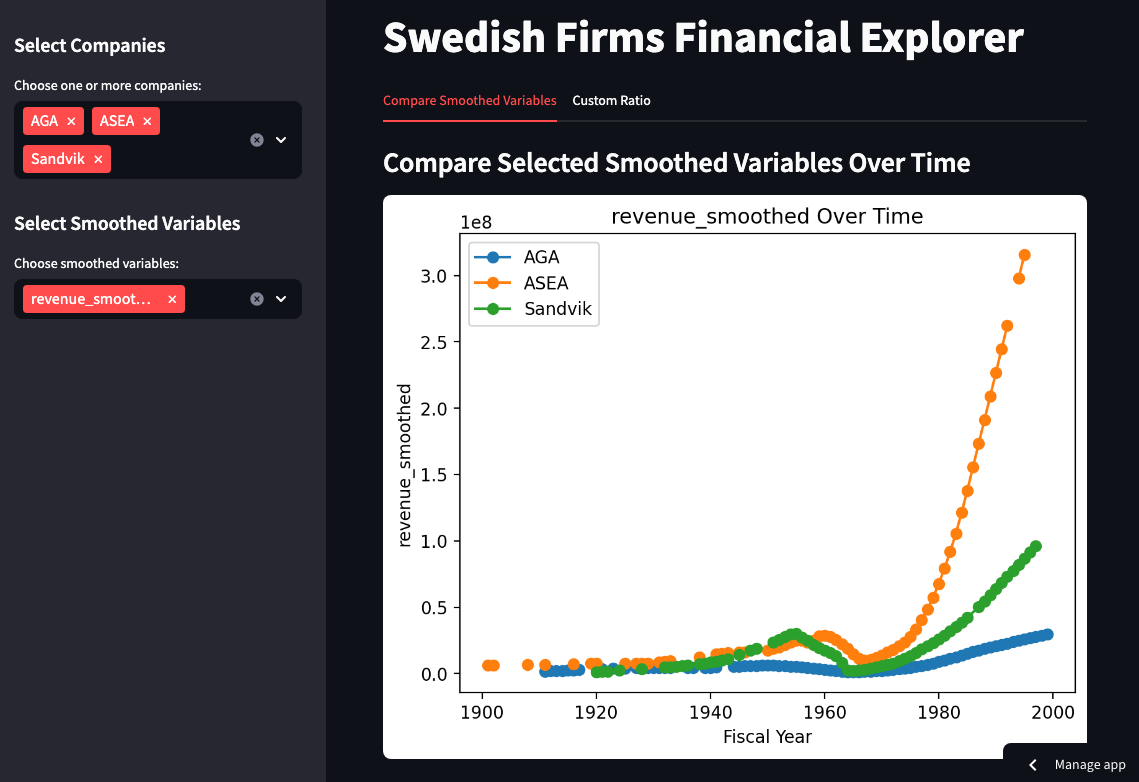
\includegraphics{images/app-01.png}

}

\subcaption{\label{fig-dp-1}First tab}

\end{minipage}%
\newline
\begin{minipage}{\linewidth}

\centering{

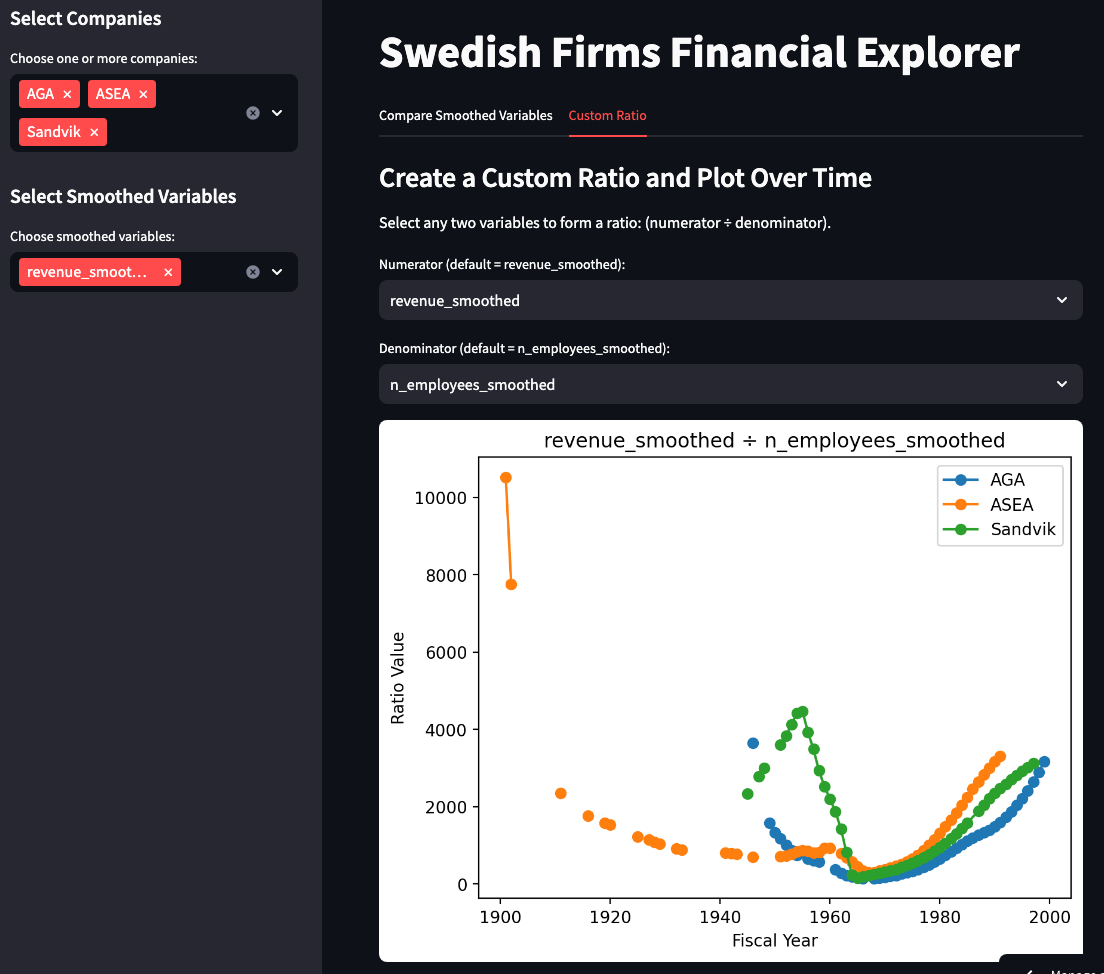
\includegraphics{images/app-02.png}

}

\subcaption{\label{fig-dp-2}Second tab}

\end{minipage}%

\caption{\label{fig-data-portal}Screenshots of the Streamlit app
interface. Source: Author's own work.}

\end{figure}%

\newpage{}

\subsection*{Works Cited}\label{works-cited}
\addcontentsline{toc}{subsection}{Works Cited}

\phantomsection\label{refs}
\begin{CSLReferences}{1}{0}
\bibitem[\citeproctext]{ref-adams2010RoleBoardsDirectors}
Adams, Renée B., Benjamin E. Hermalin, and Michael S. Weisbach. 2010.
{``The {Role} of {Boards} of {Directors} in {Corporate Governance}: {A
Conceptual Framework} and {Survey}.''} \emph{Journal of Economic
Literature} 48 (1): 58--107.
\url{https://www.jstor.org/stable/40651578}.

\bibitem[\citeproctext]{ref-asahak2018BoardsDirectorsAssessing}
Asahak, Shamiran, Simon L. Albrecht, Marcele De Sanctis, and Nicholas S.
Barnett. 2018. {``Boards of {Directors}: {Assessing Their Functioning}
and {Validation} of a {Multi-Dimensional Measure}.''} \emph{Frontiers in
Psychology} 9 (December): 2425.
\url{https://doi.org/10.3389/fpsyg.2018.02425}.

\bibitem[\citeproctext]{ref-ghardallou2020CEOCharacteristicsFirm}
Ghardallou, Wafa, Hela Borgi, and Hibah Alkhalifah. 2020. {``{CEO
Characteristics} and {Firm Performance}: {A Study} of {Saudi Arabia
Listed Firms}.''} \emph{The Journal of Asian Finance, Economics and
Business} 7 (11): 291--301.
\url{https://doi.org/10.13106/jafeb.2020.vol7.no11.291}.

\bibitem[\citeproctext]{ref-gronberg2003LearningReturningReturn}
Grönberg, Per-Olof. 2003. {``Learning and {Returning} : {Return
Migration} of {Swedish Engineers} from the {United States},
1880-1940.''} PhD thesis, Ume{å}, Faculty of Arts, Historical Studies.

\bibitem[\citeproctext]{ref-henrekson2021SocialBackgroundElite}
Henrekson, Magnus, Odd Lyssarides, and Jan Ottosson. 2021. {``The Social
Background of Elite Executives: The {Swedish} Case.''} \emph{Management
\& Organizational History} 16 (1): 65--87.
\url{https://doi.org/10.1080/17449359.2021.1950553}.

\bibitem[\citeproctext]{ref-hogfeldt2005HistoryPoliticsCorporate}
Högfeldt, Peter. 2005. {``The {History} and {Politics} of {Corporate
Ownership} in {Sweden}.''} In \emph{A History of Corporate Governance
Around the World: Family Business Groups to Professional Managers}. A
{National} Bureau of Economic Research Conference Report. Chicago:
National Bureau of Economic Research.

\bibitem[\citeproctext]{ref-jonsson2015CorporateBoardsPerformance}
Jönsson, Anna. 2015. {``Corporate {Boards} and {Performance}. {Does}
Board Composition Affect Financial Performance Among {Swedish} Firms?''}
July.

\bibitem[\citeproctext]{ref-magnusson2014SverigesEkonomiskaHistoria}
Magnusson, Lars. 2014. \emph{Sveriges Ekonomiska Historia}. Lund:
Studentlitteratur.

\bibitem[\citeproctext]{ref-prado2022ModernSwedishEconomic}
Prado, Svante, and Jakob Molinder. 2022. {``Modern {Swedish Economic
History}.''} In \emph{Oxford {Research Encyclopedia} of {Economics} and
{Finance}}. Oxford University Press.
\url{https://doi.org/10.1093/acrefore/9780190625979.013.679}.

\bibitem[\citeproctext]{ref-sabelfeld2023SwedishCorporateGovernance}
Sabelfeld, Svetlana, and Kristina Jonäll. 2023. {``The {Swedish}
Corporate Governance Setting.''} In \emph{Corporate {Governance} in a
{Nordic Setting}}, 53--62. De Gruyter.
\url{https://doi.org/10.1515/9783110725346-005}.

\bibitem[\citeproctext]{ref-sluyterman2022ChangingRoleCEOs}
Sluyterman, Keetie, and Gerarda Westerhuis. 2022. {``The {Changing Role}
of {CEOs} in {Dutch Listed Companies}, 1957--2007.''} \emph{Enterprise
\& Society} 23 (3): 711--45. \url{https://doi.org/10.1017/eso.2020.77}.

\bibitem[\citeproctext]{ref-taalbiInnovationsEconomicGrowth}
Taalbi, Josef, and Jonas Ljungberg. n.d. {``Innovations and {Economic
Growth} in the {Swedish Engineering Industry}, 1914-2013.''} In
\emph{Eleventh {Conference} of the {European Historical Economics
Society}, {Pisa} 4-5 {September}, 2015}.

\bibitem[\citeproctext]{ref-vonmeyerinck2016DirectorIndustryExperience}
von Meyerinck, Felix, David Oesch, and Markus Schmid. 2016. {``Is
{Director Industry Experience Valuable}?''} \emph{Financial Management}
45 (1): 207--37. \url{https://www.jstor.org/stable/24736522}.

\end{CSLReferences}




\end{document}
